\documentclass[aspectratio=169,11pt]{beamer}
% ==========================================================================
%  KSA lecture-slide theme  =  stock beamer "Boadilla"  +  KSA colour theme
%  brand colours sampled from the official KSA symbol mark:
%    Deep Prussian Blue  #2E3192   (지성 - intellect)
%    Golden Gray         #D6CBB1   (감성 - sensibility)
%  Engine: XeLaTeX.  Usage:
%    \documentclass[aspectratio=169,11pt]{beamer}
%    % ==========================================================================
%  KSA lecture-slide theme  =  stock beamer "Boadilla"  +  KSA colour theme
%  brand colours sampled from the official KSA symbol mark:
%    Deep Prussian Blue  #2E3192   (지성 - intellect)
%    Golden Gray         #D6CBB1   (감성 - sensibility)
%  Engine: XeLaTeX.  Usage:
%    \documentclass[aspectratio=169,11pt]{beamer}
%    % ==========================================================================
%  KSA lecture-slide theme  =  stock beamer "Boadilla"  +  KSA colour theme
%  brand colours sampled from the official KSA symbol mark:
%    Deep Prussian Blue  #2E3192   (지성 - intellect)
%    Golden Gray         #D6CBB1   (감성 - sensibility)
%  Engine: XeLaTeX.  Usage:
%    \documentclass[aspectratio=169,11pt]{beamer}
%    \input{../theme/ksa-theme.tex}
% ==========================================================================

\usepackage{fontspec}
\usepackage{amsmath,amssymb}
\usepackage{graphicx}
\graphicspath{{figs/}{../figs/}}
\usepackage{booktabs}
\usepackage{listings}

% ---- fonts (no ctex/xeCJK on this box -> fontspec drives CJK directly) -----
\defaultfontfeatures{Ligatures=TeX}
\setmainfont{Noto Sans CJK KR}
\setsansfont{Noto Sans CJK KR}
\setmonofont{Noto Sans Mono CJK KR}[Scale=0.92]

% ---- base theme: stock Boadilla ------------------------------------------
\usetheme{Boadilla}
\usefonttheme{professionalfonts}
\setbeamertemplate{navigation symbols}{}

% ---- KSA colour theme (recolour the stock theme) --------------------------
\definecolor{ksablue}{HTML}{2E3192}
\definecolor{ksabluedk}{HTML}{20226A}
\definecolor{ksagold}{HTML}{D6CBB1}
\definecolor{ksagolddk}{HTML}{A9976B}
\definecolor{ksared}{HTML}{C0392B}
\definecolor{ksagray}{HTML}{5B5B5B}

\setbeamercolor{structure}{fg=ksablue}
\setbeamercolor{alerted text}{fg=ksared}

\setbeamercolor{palette primary}{fg=white,           bg=ksablue}
\setbeamercolor{palette secondary}{fg=white,         bg=ksablue!85!black}
\setbeamercolor{palette tertiary}{fg=white,          bg=ksabluedk}
\setbeamercolor{titlelike}{fg=ksablue}
\setbeamercolor{frametitle}{fg=ksablue,bg=}
\setbeamercolor{title}{fg=ksablue}
\setbeamercolor{author}{fg=ksagray}
\setbeamercolor{institute}{fg=ksagray}
\setbeamercolor{block title}{fg=white,bg=ksablue}
\setbeamercolor{block body}{fg=black!85,bg=ksablue!6}
\setbeamercolor{item}{fg=ksablue}
\setbeamercolor{section in toc}{fg=black!85}

\setbeamerfont{frametitle}{series=\bfseries}
\setbeamerfont{title}{series=\bfseries}

% ---- footline:  KSA mark | "Made by ..." | n / N   (matches reference) ----
\newcommand{\ksacredit}{Made by Sumin Han \,\textperiodcentered\, suminhan@ksa.hs.kr}
\setbeamertemplate{footline}{%
  \hbox{%
    \begin{beamercolorbox}[wd=.18\paperwidth,ht=2.6ex,dp=1.5ex,leftskip=1.1em]{}%
      \raisebox{-0.35ex}{
\includegraphics[height=2.0ex]{ksa-logo.png}}%
    \end{beamercolorbox}%
    \begin{beamercolorbox}[wd=.64\paperwidth,ht=2.6ex,dp=1.5ex,center]{}%
      {\scriptsize\color{ksagray}\ksacredit}%
    \end{beamercolorbox}%
    \begin{beamercolorbox}[wd=.18\paperwidth,ht=2.6ex,dp=1.5ex,rightskip=1.1em]{}%
      \hfill{\scriptsize\color{ksablue}\insertframenumber\,/\,\inserttotalframenumber}%
    \end{beamercolorbox}%
  }%
  \vskip2pt
}

% ---- section divider: stock \sectionpage, KSA-coloured -------------------
\setbeamertemplate{section page}{%
  \begingroup\centering
    {\color{ksagolddk}\rule{0.16\paperwidth}{1pt}}\par\vskip1.0em
    {\usebeamerfont{title}\color{ksablue}\insertsectionhead\par}\vskip1.0em
    {\color{ksagolddk}\rule{0.16\paperwidth}{1pt}}\par
  \endgroup
}
\AtBeginSection[]{\begin{frame}[plain,noframenumbering]\vfill\sectionpage\vfill\end{frame}}

% ---- code listings ------------------------------------------------------------
\lstdefinestyle{ksa}{%
  basicstyle=\ttfamily\scriptsize,
  keywordstyle=\color{ksablue}\bfseries,
  commentstyle=\color{ksagray}\itshape,
  stringstyle=\color{ksagolddk},
  numberstyle=\tiny\color{ksagray},
  backgroundcolor=\color{ksablue!6},
  frame=leftline, framerule=1.4pt, rulecolor=\color{ksablue},
  xleftmargin=1em, aboveskip=0.8em, belowskip=0.4em,
  showstringspaces=false, breaklines=true, language=Python,
}
\lstset{style=ksa}

% ---- handy macros -----------------------------------------------------------
\newcommand{\kb}[1]{\textbf{\color{ksablue}#1}}   % blue keyword
\newcommand{\kq}[1]{\textbf{\color{ksared}#1}}    % red key-question

% ==========================================================================

\usepackage{fontspec}
\usepackage{amsmath,amssymb}
\usepackage{graphicx}
\graphicspath{{figs/}{../figs/}}
\usepackage{booktabs}
\usepackage{listings}

% ---- fonts (no ctex/xeCJK on this box -> fontspec drives CJK directly) -----
\defaultfontfeatures{Ligatures=TeX}
\setmainfont{Noto Sans CJK KR}
\setsansfont{Noto Sans CJK KR}
\setmonofont{Noto Sans Mono CJK KR}[Scale=0.92]

% ---- base theme: stock Boadilla ------------------------------------------
\usetheme{Boadilla}
\usefonttheme{professionalfonts}
\setbeamertemplate{navigation symbols}{}

% ---- KSA colour theme (recolour the stock theme) --------------------------
\definecolor{ksablue}{HTML}{2E3192}
\definecolor{ksabluedk}{HTML}{20226A}
\definecolor{ksagold}{HTML}{D6CBB1}
\definecolor{ksagolddk}{HTML}{A9976B}
\definecolor{ksared}{HTML}{C0392B}
\definecolor{ksagray}{HTML}{5B5B5B}

\setbeamercolor{structure}{fg=ksablue}
\setbeamercolor{alerted text}{fg=ksared}

\setbeamercolor{palette primary}{fg=white,           bg=ksablue}
\setbeamercolor{palette secondary}{fg=white,         bg=ksablue!85!black}
\setbeamercolor{palette tertiary}{fg=white,          bg=ksabluedk}
\setbeamercolor{titlelike}{fg=ksablue}
\setbeamercolor{frametitle}{fg=ksablue,bg=}
\setbeamercolor{title}{fg=ksablue}
\setbeamercolor{author}{fg=ksagray}
\setbeamercolor{institute}{fg=ksagray}
\setbeamercolor{block title}{fg=white,bg=ksablue}
\setbeamercolor{block body}{fg=black!85,bg=ksablue!6}
\setbeamercolor{item}{fg=ksablue}
\setbeamercolor{section in toc}{fg=black!85}

\setbeamerfont{frametitle}{series=\bfseries}
\setbeamerfont{title}{series=\bfseries}

% ---- footline:  KSA mark | "Made by ..." | n / N   (matches reference) ----
\newcommand{\ksacredit}{Made by Sumin Han \,\textperiodcentered\, suminhan@ksa.hs.kr}
\setbeamertemplate{footline}{%
  \hbox{%
    \begin{beamercolorbox}[wd=.18\paperwidth,ht=2.6ex,dp=1.5ex,leftskip=1.1em]{}%
      \raisebox{-0.35ex}{
\includegraphics[height=2.0ex]{ksa-logo.png}}%
    \end{beamercolorbox}%
    \begin{beamercolorbox}[wd=.64\paperwidth,ht=2.6ex,dp=1.5ex,center]{}%
      {\scriptsize\color{ksagray}\ksacredit}%
    \end{beamercolorbox}%
    \begin{beamercolorbox}[wd=.18\paperwidth,ht=2.6ex,dp=1.5ex,rightskip=1.1em]{}%
      \hfill{\scriptsize\color{ksablue}\insertframenumber\,/\,\inserttotalframenumber}%
    \end{beamercolorbox}%
  }%
  \vskip2pt
}

% ---- section divider: stock \sectionpage, KSA-coloured -------------------
\setbeamertemplate{section page}{%
  \begingroup\centering
    {\color{ksagolddk}\rule{0.16\paperwidth}{1pt}}\par\vskip1.0em
    {\usebeamerfont{title}\color{ksablue}\insertsectionhead\par}\vskip1.0em
    {\color{ksagolddk}\rule{0.16\paperwidth}{1pt}}\par
  \endgroup
}
\AtBeginSection[]{\begin{frame}[plain,noframenumbering]\vfill\sectionpage\vfill\end{frame}}

% ---- code listings ------------------------------------------------------------
\lstdefinestyle{ksa}{%
  basicstyle=\ttfamily\scriptsize,
  keywordstyle=\color{ksablue}\bfseries,
  commentstyle=\color{ksagray}\itshape,
  stringstyle=\color{ksagolddk},
  numberstyle=\tiny\color{ksagray},
  backgroundcolor=\color{ksablue!6},
  frame=leftline, framerule=1.4pt, rulecolor=\color{ksablue},
  xleftmargin=1em, aboveskip=0.8em, belowskip=0.4em,
  showstringspaces=false, breaklines=true, language=Python,
}
\lstset{style=ksa}

% ---- handy macros -----------------------------------------------------------
\newcommand{\kb}[1]{\textbf{\color{ksablue}#1}}   % blue keyword
\newcommand{\kq}[1]{\textbf{\color{ksared}#1}}    % red key-question

% ==========================================================================

\usepackage{fontspec}
\usepackage{amsmath,amssymb}
\usepackage{graphicx}
\graphicspath{{figs/}{../figs/}}
\usepackage{booktabs}
\usepackage{listings}

% ---- fonts (no ctex/xeCJK on this box -> fontspec drives CJK directly) -----
\defaultfontfeatures{Ligatures=TeX}
\setmainfont{Noto Sans CJK KR}
\setsansfont{Noto Sans CJK KR}
\setmonofont{Noto Sans Mono CJK KR}[Scale=0.92]

% ---- base theme: stock Boadilla ------------------------------------------
\usetheme{Boadilla}
\usefonttheme{professionalfonts}
\setbeamertemplate{navigation symbols}{}

% ---- KSA colour theme (recolour the stock theme) --------------------------
\definecolor{ksablue}{HTML}{2E3192}
\definecolor{ksabluedk}{HTML}{20226A}
\definecolor{ksagold}{HTML}{D6CBB1}
\definecolor{ksagolddk}{HTML}{A9976B}
\definecolor{ksared}{HTML}{C0392B}
\definecolor{ksagray}{HTML}{5B5B5B}

\setbeamercolor{structure}{fg=ksablue}
\setbeamercolor{alerted text}{fg=ksared}

\setbeamercolor{palette primary}{fg=white,           bg=ksablue}
\setbeamercolor{palette secondary}{fg=white,         bg=ksablue!85!black}
\setbeamercolor{palette tertiary}{fg=white,          bg=ksabluedk}
\setbeamercolor{titlelike}{fg=ksablue}
\setbeamercolor{frametitle}{fg=ksablue,bg=}
\setbeamercolor{title}{fg=ksablue}
\setbeamercolor{author}{fg=ksagray}
\setbeamercolor{institute}{fg=ksagray}
\setbeamercolor{block title}{fg=white,bg=ksablue}
\setbeamercolor{block body}{fg=black!85,bg=ksablue!6}
\setbeamercolor{item}{fg=ksablue}
\setbeamercolor{section in toc}{fg=black!85}

\setbeamerfont{frametitle}{series=\bfseries}
\setbeamerfont{title}{series=\bfseries}

% ---- footline:  KSA mark | "Made by ..." | n / N   (matches reference) ----
\newcommand{\ksacredit}{Made by Sumin Han \,\textperiodcentered\, suminhan@ksa.hs.kr}
\setbeamertemplate{footline}{%
  \hbox{%
    \begin{beamercolorbox}[wd=.18\paperwidth,ht=2.6ex,dp=1.5ex,leftskip=1.1em]{}%
      \raisebox{-0.35ex}{
\includegraphics[height=2.0ex]{ksa-logo.png}}%
    \end{beamercolorbox}%
    \begin{beamercolorbox}[wd=.64\paperwidth,ht=2.6ex,dp=1.5ex,center]{}%
      {\scriptsize\color{ksagray}\ksacredit}%
    \end{beamercolorbox}%
    \begin{beamercolorbox}[wd=.18\paperwidth,ht=2.6ex,dp=1.5ex,rightskip=1.1em]{}%
      \hfill{\scriptsize\color{ksablue}\insertframenumber\,/\,\inserttotalframenumber}%
    \end{beamercolorbox}%
  }%
  \vskip2pt
}

% ---- section divider: stock \sectionpage, KSA-coloured -------------------
\setbeamertemplate{section page}{%
  \begingroup\centering
    {\color{ksagolddk}\rule{0.16\paperwidth}{1pt}}\par\vskip1.0em
    {\usebeamerfont{title}\color{ksablue}\insertsectionhead\par}\vskip1.0em
    {\color{ksagolddk}\rule{0.16\paperwidth}{1pt}}\par
  \endgroup
}
\AtBeginSection[]{\begin{frame}[plain,noframenumbering]\vfill\sectionpage\vfill\end{frame}}

% ---- code listings ------------------------------------------------------------
\lstdefinestyle{ksa}{%
  basicstyle=\ttfamily\scriptsize,
  keywordstyle=\color{ksablue}\bfseries,
  commentstyle=\color{ksagray}\itshape,
  stringstyle=\color{ksagolddk},
  numberstyle=\tiny\color{ksagray},
  backgroundcolor=\color{ksablue!6},
  frame=leftline, framerule=1.4pt, rulecolor=\color{ksablue},
  xleftmargin=1em, aboveskip=0.8em, belowskip=0.4em,
  showstringspaces=false, breaklines=true, language=Python,
}
\lstset{style=ksa}

% ---- handy macros -----------------------------------------------------------
\newcommand{\kb}[1]{\textbf{\color{ksablue}#1}}   % blue keyword
\newcommand{\kq}[1]{\textbf{\color{ksared}#1}}    % red key-question


\title{고급 정책 최적화: PPO (Proximal Policy Optimization)}
\subtitle{신뢰 영역과 확률비 \,$\cdot$\, PPO 클리핑과 연속 제어 실습 \,$\cdot$\, GAE와 PPO가 표준이 된 이유}
\author{Machine Learning 2 \,\textperiodcentered\, 11주차}
\institute{한국과학영재학교 (KSA)}
\date{Chapter 11}

\begin{document}

% ===== title =====
\begin{frame}[plain,noframenumbering]
  \titlepage
\end{frame}

% ===== overview of this week =====
\begin{frame}{이번 주차 개요}
  \small
  \begin{columns}[T]
    \begin{column}{0.58\textwidth}
      \textbf{이 챕터를 마치면}
      \begin{itemize}
        \item \kb{신뢰 영역}의 뜻 — 한 업데이트에서 정책이 움직일 수
          있는 크기를 KL 발산으로 잰 ``믿을 수 있는 범위''로 제한하는 것.
        \item $L^{\mathrm{IS}}(\theta)=\mathbb{E}_t[r_t(\theta)A_t]$ 의
          그래디언트가 $r_t=1$ 에서 평범한 정책 그래디언트와
          \textbf{정확히 같아지는 것}을 유도.
        \item $L^{\mathrm{CLIP}}$ 의 모양을 손으로 그려, min이 만드는
          모서리가 \textbf{개선 방향에만} 그래디언트를 0으로 만드는
          비대칭을 설명.
        \item \kb{GAE}(TD 오차를 지수적으로 가중합, $\lambda$ 로 TD와
          MC 사이를 절충)와 엔트로피 보너스가 왜 필요한지 설명.
        \item PPO 한 반복 전체 데이터 흐름을 따라가고, 연속 제어
          (Pendulum)에서 PPO를 학습시킬 수 있다.
      \end{itemize}
    \end{column}
    \begin{column}{0.40\textwidth}
      \kb{11.1} 신뢰 영역과 확률비 — 클리핑의 ``재료'' 준비.
      \\[0.5em]
      \kb{11.2} PPO 클리핑과 연속 제어 실습 — 한 줄의 식이 만드는
      목적함수의 모양 + Pendulum 실습.
      \\[0.5em]
      \kb{11.3} GAE와 PPO가 표준이 된 이유 — 실전용 마지막 두 조각,
      TRPO 비교, 전체 스택.
    \end{column}
  \end{columns}
\end{frame}

\section{11.1 신뢰 영역과 확률비}

\begin{frame}{위치: 이번 절이 해결할 문제}
  Chapter 10의 REINFORCE와 Actor-Critic에 공통된 한계 두 가지.
  \vskip0.6em
  \begin{itemize}
    \item \kb{문제 1 — 데이터 한 번 쓰고 버린다.} 에피소드 한 번
      모은 데이터를 그 자리에서 바로 쓰면 (온-폴리시, on-policy),
      정책이 바뀌는 순간 ``옛 정책이 그 행동을 얼마나 좋아했는가''
      기반의 그래디언트는 더 이상 정확하지 않다.
    \item \kb{문제 2 — 스텝이 한 번이라도 너무 크면.} 정책이 갑자기
      나쁜 방향으로 확 바뀌어 이후 돌려놓기 어렵다. 로봇처럼
      ``한 번 무너지면 다시 세우기 어렵다''는 상황에서는 치명적.
  \end{itemize}
  \vskip0.6em
  \begin{block}{이번 절의 두 도구}
    \kb{신뢰 영역}(trust region): 한 번의 업데이트에서 정책이 얼마나
    움직일 수 있는가의 상한. \kb{확률비}(probability ratio): 옛 정책
    데이터의 재사용을 가능하게 하는 도구. 이 둘이 11.2절에서
    \textbf{클리핑} 한 줄로 합쳐진다.
  \end{block}
\end{frame}

\begin{frame}{신뢰 영역이라는 직관}
  \begin{columns}[T]
    \begin{column}{0.55\textwidth}
      \kb{산에서 안개 낀 내리막}
      \begin{itemize}
        \item 한 치 앞만 보이는 안개 속에서, 가장 가파른 방향으로
          무작정 큰 걸음을 내디디면 절벽으로 떨어질 수 있다.
        \item 안전한 전략: \textbf{한 걸음의 크기를 ``믿을 수 있는
          범위''(신뢰 영역) 안으로 제한}.
        \item 매 스텝이 실제로 개선을 보장하는 좁은 범위 안에서만
          이동하게 한다 — 이것이 PPO의 핵심 아이디어.
      \end{itemize}
      \vskip0.6em
      \kq{``한 걸음의 크기''는 어떻게 재는가?}
      \smallskip
      \small
      정책은 행동의 \textbf{확률분포}이므로, 파라미터의 차
      $\lVert\theta-\theta_{\mathrm{old}}\rVert$ 로 재기보다
      \textbf{분포 자체의 거리}로 재는 것이 자연스럽다.
    \end{column}
    \begin{column}{0.43\textwidth}
      \kb{표준적인 선택: KL 발산}
      \[
      D_{\mathrm{KL}}(\pi_\theta\,\|\,\pi_{\theta_{\mathrm{old}}})
      = \mathbb{E}_{s\sim\rho}\Big[\,
      \mathbb{E}_{a\sim\pi_\theta(\cdot\mid s)}
      \log\frac{\pi_\theta(a\mid s)}
      {\pi_{\theta_{\mathrm{old}}}(a\mid s)}\Big]
      \]
      {\footnotesize $\rho$ = 상태 방문 분포. 0이면 두 정책이
      정확히 같고, 클수록 서로 다른 행동을 다르게 선호 —
      ``정책 공간에서의 걸음 크기''를 재는 눈금.}
    \end{column}
  \end{columns}
\end{frame}

\begin{frame}{TRPO: 보장은 강력, 기계는 무거움}
  \begin{itemize}
    \item \kb{TRPO(Trust Region Policy Optimization, 2015)}:
      ``KL 발산이 $\delta$ 를 넘지 않는 범위 안에서 $J(\theta)$ 를
      최대화한다''는 \textbf{제약된 최적화}를 매 스텝마다 풀었다.
    \item \kb{보장}: 제약이 충분히 작으면 매 업데이트가 성능을 절대
      떨어뜨리지 않는 \textbf{단조 개선}을 증명.
    \item \kb{대가}: 실제로 이 제약을 풀려면
      \begin{itemize}
        \item 2차 미분 — \kb{피셔 정보 행렬}
        \item 역행렬 곱을 반복적으로 — \kb{conjugate gradient}
        \item 제안 방향으로 얼마나 가도 안전한지 — \kb{line search}
      \end{itemize}
      \textbf{세 장치}까지 동원해야 해서 무겁다.
  \end{itemize}
  \vskip0.4em
  {\small PPO의 출발 질문: ``이 강력한 보장을 유지하면서 이
  기계장치를 어떻게 단순화할 수 있는가?'' — 단순화의 핵심이 바로
  확률비.}
\end{frame}

\begin{frame}[fragile]{TRPO의 데이터 생성 절차 (원 논문 Figure 1)}
  \begin{columns}[T]
    \begin{column}{0.62\textwidth}
      \centering
      
\includegraphics[width=\linewidth]{ref_trpo.png}
    \end{column}
    \begin{column}{0.36\textwidth}
      {\small
      \kb{single path} (좌): 시뮬레이션한 단일 트래젝터리의 모든
      상태-행동 쌍을 목적함수에 사용.
      \\[0.8em]
      \kb{vine} (우): 줄기(trunk) 트래젝터리의 도달 상태 일부에서
      가지(branch) 롤아웃을 퍼뜨림 (공통 무작위 수) — 분산 감소
      효과.
      \\[0.8em]
      TRPO의 무거움은 ``이 데이터에 어떤 최적화 장치를
      붙이느냐''의 문제에서 온다.
      }
    \end{column}
  \end{columns}
\end{frame}

\begin{frame}{확률비와 중요도 샘플링}
  핵심 도구 — \kb{확률비}(probability ratio): 지금 업데이트하려는
  정책 $\pi_\theta$ 와 데이터를 모을 때 썼던 정책
  $\pi_{\theta_{\mathrm{old}}}$ 가 \textbf{같은 행동}에 부여하는
  확률의 비.
  \[
  r_t(\theta) := \frac{\pi_\theta(a_t\mid s_t)}
  {\pi_{\theta_{\mathrm{old}}}(a_t\mid s_t)},
  \quad r_t(\theta_{\mathrm{old}}) = 1
  \]
  \begin{itemize}
    \item $r_t > 1$: 그 행동을 전보다 \textbf{더} 선호.
      \; $r_t < 1$: \textbf{덜} 선호.
    \item 이 비율로 ``옛 정책이 모은 데이터''를 ``새 정책
      관점에서'' 재사용 — \kb{중요도 샘플링}(Chapter 5.3의
      MC off-policy 학습에서 처음 등장한 바로 그 도구).
  \end{itemize}
  \[
  L^{\mathrm{IS}}(\theta) = \mathbb{E}_t[\,r_t(\theta)\, A_t\,]
  \]
  $A_t$ 는 10.3절의 어드밴티지 $A_t := G_t - V(s_t)$.
\end{frame}

\begin{frame}{그냥 최대화하면 폭주 — 그리고 그래디언트}
  \begin{itemize}
    \item $L^{\mathrm{IS}}$ 를 그냥 최대화하면 $r_t$ 가 한없이
      커지도록 (같은 행동만 계속 더 밀어주도록) 학습이 \textbf{폭주}
      — 데이터는 재사용되지만 ``정책이 너무 멀리 움직이지 않는다''는
      보장은 어디에도 없다.
  \end{itemize}
  \vskip0.5em
  \kq{왜 $L^{\mathrm{IS}}$ 를 최대화하면 원래 목표 $J(\theta)$ 를
  최대화하는 것과 같은 방향인가?}
  \small
  $\pi_{\mathrm{old}}$ 는 $\theta$ 와 무관한 상수(데이터 수집 때
  고정했던 정책)이므로:
  \[
  \nabla_\theta L^{\mathrm{IS}}
  = \mathbb{E}_t\Big[\frac{\pi_\theta}{\pi_{\mathrm{old}}}\,
  \nabla_\theta\log\pi_\theta\, A_t\Big]
  = \mathbb{E}_t[\,r_t(\theta)\,\nabla_\theta\log\pi_\theta\, A_t\,]
  \]
  두 번째 등호는 10.1절 \kb{로그미분 트릭}
  ($\nabla\pi = \pi\nabla\log\pi$)의 직접 적용.
\end{frame}

\begin{frame}{첫 스텝에서는 ``정직한 첫 걸음''}
  \begin{block}{핵심 성립}
    $L^{\mathrm{IS}}$ 의 그래디언트는 \textbf{평범한 policy gradient
    $\nabla_\theta\log\pi_\theta\, A_t$ 에 계수 $r_t$ 가 곱해진
    형태}다. 데이터를 방금 모은 시점
    ($\theta=\theta_{\mathrm{old}}$)에서는 $r_t=1$ 이므로
    \textbf{10.3절 Actor-Critic의 그래디언트와 정확히 같다}.
  \end{block}
  \vskip0.5em
  \begin{itemize}
    \item 즉, 확률비로 목적함수를 다시 쓴 순간
      \kb{``옛 데이터를 재사용해도 첫 스텝에서는 정직한 policy
      gradient''}가 자동으로 성립 — 이것이 확률비가 ``재사용의
      열쇠''인 이유.
    \item $\theta$ 가 $\theta_{\mathrm{old}}$ 에서 멀어지면 계수
      $r_t$ 가 1에서 벗어나 이 동등성이 \textbf{약해진다} —
      ``멀어지는 정도''를 막는 것이 11.2절의 클리핑.
  \end{itemize}
\end{frame}

\begin{frame}{손으로 한번: $r_t$ 는 실제로 어떻게 움직이는가}
  2-행동 softmax 정책, 로짓 $(\theta_0,\theta_1)$.
  시작점 $\theta_{\mathrm{old}}=(0,0)$ 에서 두 행동 반반
  ($p_0=0.5$). ``행동 0이 좋다''며 $\theta_0$ 를 계속 올리고
  $\theta_1=0$ 을 고정하면:
  \vskip0.6em
  \small
  \begin{tabular}{@{}lll@{}}
    \toprule
    $\theta$ & $p_0$ (새 정책) & $r_0 = p_0/0.5$ \\
    \midrule
    $(0.0,\,0.0)$ & 0.5000 & \textbf{1.000} (처음) \\
    $(1.1,\,0.0)$ & 0.7503 & 1.501 \\
    $(2.2,\,0.0)$ & 0.9002 & 1.800 \\
    $(4.4,\,0.0)$ & 0.9879 & 1.976 \\
    \bottomrule
  \end{tabular}
  \vskip0.8em
  \small
  세 가지가 보인다:
  \begin{enumerate}
    \item $r_0$ 는 항상 \textbf{1에서 출발} (데이터 수집 시점에는
      새·옛 정책이 같으므로).
    \item 좋은 행동을 계속 밀면 $r_0$ 가 1보다 커지며 \textbf{오르
      다} — ``더 선호하게 됐다''의 정량.
    \item 이산 정책은 $p_0\le 1$ 이므로 $r_0\le 2$ —
      \textbf{위에서 유한}. 다만 경계(2)에 빠르게 붙는다.
  \end{enumerate}
  {\footnotesize 클리핑(11.2)이 막는 것은 정확히 이 ``경계에
  붙는'' 구간: $r_0>1.2$ 이후엔 목적함수에 기여 0, $p_0$ 가 0.9
  이상으로 확 밀리는 것을 허용하지 않음.}
\end{frame}

\begin{frame}{연속 정책: $r_t$ 의 분산이 지수적으로 불어난다}
  이산 2-행동에서는 유한했지만, ``$r_t$ 가 커지면?'' —
  \kb{중요도 샘플링의 분산}이 문제. 가장 단순한 연속 사례:
  같은 $\sigma=1$ 인 가우시안 정책 둘,
  $\pi_{\mathrm{old}}=\mathcal{N}(0,1)$,
  $\pi_\theta=\mathcal{N}(\mu,1)$ (평균만 $\mu$ 이동).
  \small
  \[
  r(x) = \frac{\pi_\theta(x)}{\pi_{\mathrm{old}}(x)}
  = \exp\Big(-\tfrac{x^2}{2}+\tfrac{(x-\mu)^2}{2}\Big)
  = \exp\Big(\mu x - \tfrac{\mu^2}{2}\Big)
  \]
  \begin{itemize}
    \item 이것은 \kb{로그정규분포}. 기댓값은 항상 1(재가중해도
      평균 보존).
    \item \textbf{분산}은 $\operatorname{Var}[r]=e^{\mu^2}-1$ —
      $\mu^2$ 에 \textbf{지수적으로} 불어난다.
  \end{itemize}
\end{frame}

\begin{frame}{μ를 세 배로, 분산은 사천 배}
  \small
  \begin{tabular}{@{}rrrr@{}}
    \toprule
    평균 이동 $\mu$ & $\operatorname{Var}[r]=e^{\mu^2}-1$ &
      $\Pr(r>5)$ & $r$ 의 99퍼센타일 \\
    \midrule
    0.5 & 0.284 & 0.00026 & 3.6 \\
    1.0 & 1.718 & 0.0175 & 16.9 \\
    1.5 & 8.488 & 0.0342 & 100.9 \\
    2.0 & 53.598 & 0.0356 & 774.8 \\
    2.5 & 517.013 & 0.0291 & 7636.9 \\
    3.0 & 8102.084 & 0.0209 & 96654.7 \\
    \bottomrule
  \end{tabular}
  \vskip0.6em
  \begin{itemize}
    \item $\mu=1$ 이면 분산 1.7 (아직 괜찮아 보인다)
      $\to$ $\mu=2$ 이면 53.6 $\to$ $\mu=3$ 이면 \textbf{8102}.
    \item ``새 정책이 옛 정책과 살짝 다를 뿐''이라고 느긋하게 넘길
      수 없는 구간.
  \end{itemize}
\end{frame}

\begin{frame}{소수 극단 샘플이 업데이트를 지배한다}
  \begin{columns}[T]
    \begin{column}{0.60\textwidth}
      \centering
      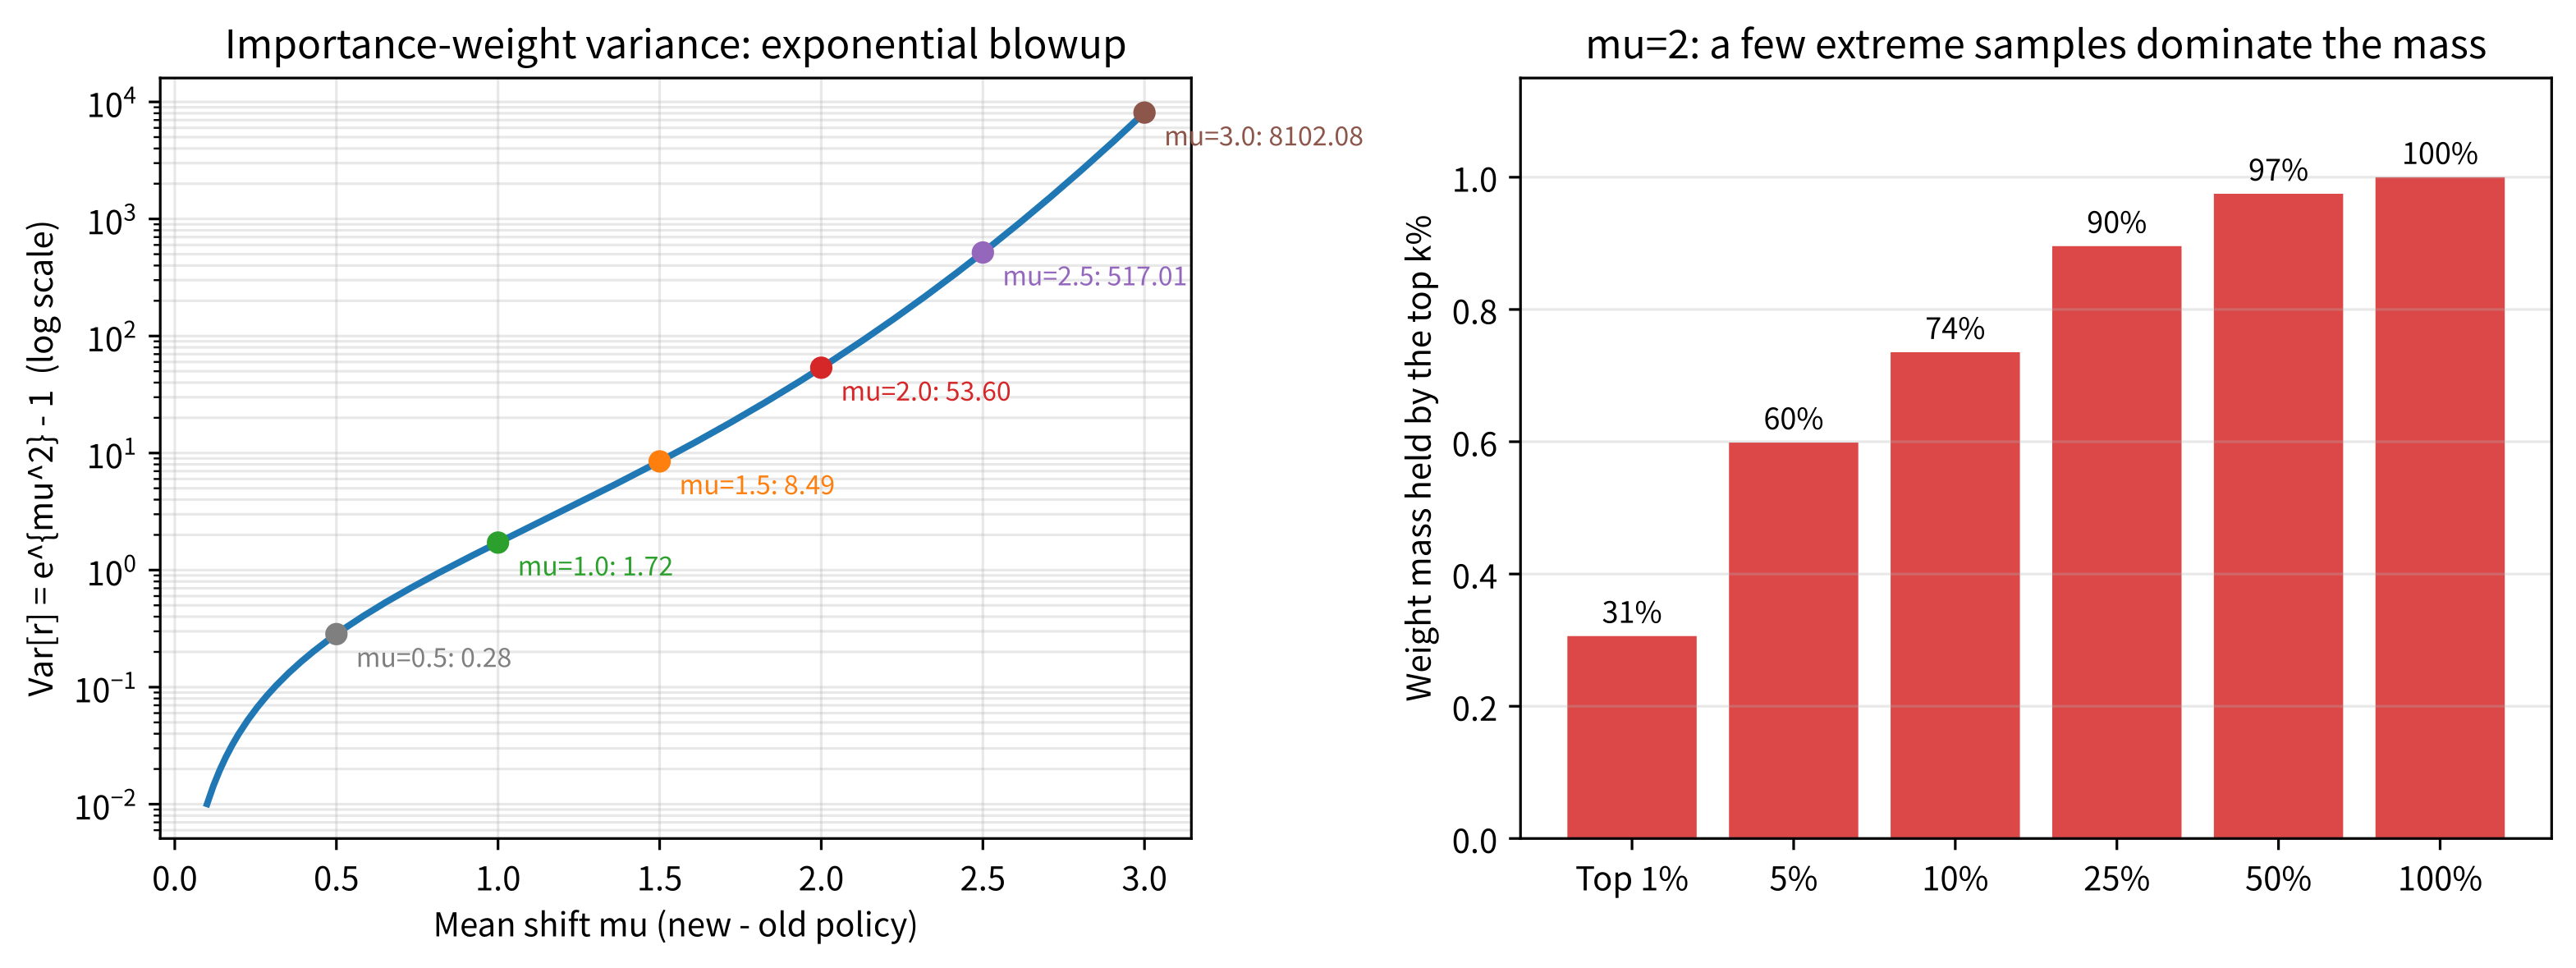
\includegraphics[width=\linewidth]{ch11_1_ratio_variance.png}
      {\footnotesize 좌: $\mu$ 이동에 따른 $\operatorname{Var}[r]
      =e^{\mu^2}-1$ (로그 축). 우: $\mu=2$ 일 때 10,000개 샘플 중
      상위 1\%가 전체 가중치 합의 약 31\% 차지.}
    \end{column}
    \begin{column}{0.38\textwidth}
      {\small
      $\mu=2$ 로 10,000개 샘플:
      \begin{itemize}
        \item 가중치 평균은 1에 가까움 (0.91).
        \item \textbf{최댓값은 약 143}.
        \item \textbf{상위 1\%(100개)} 샘플이 전체 가중치 합에서
          약 \textbf{31\%} 차지.
      \end{itemize}
      }
      \vskip0.5em
      {\small 업데이트 방향을 정하는 것은 ``대부분의 샘플''이
      아니라 \textbf{소수의 극단 샘플} — 극단 샘플이 노이즈이므로
      업데이트가 노이즈에 지배당해 정책이 흔들린다.
      바로 11.2절 클리핑이 ``극단 샘플의 기여를
      $1+\epsilon$ 으로 잘라버리는'' 이유.}
    \end{column}
  \end{columns}
\end{frame}

\begin{frame}{``분산이 크다'' $\neq$ ``한 샘플이 지배한다''}
  \kq{분산이 큰 것과 한 샘플이 지배하는 것은 같은 말인가?}
  관련되지만 \textbf{다르고, 여기서는 둘 다} 문제가 된다.
  \vskip0.6em
  \begin{columns}[T]
    \begin{column}{0.48\textwidth}
      \kb{분산이 크다}
      \begin{itemize}
        \item \textbf{반복 평균}으로 (데이터를 많이 모으면)
          줄여줄 수 있다.
      \end{itemize}
    \end{column}
    \begin{column}{0.48\textwidth}
      \kb{단일 스텝에서 한 샘플이 지배한다}
      \begin{itemize}
        \item 데이터량이 충분해도, 극단 샘플이 *한 방향*으로 운
          좋게 쏠리면 \textbf{그 한 스텝이 크게 틀어진다}.
      \end{itemize}
    \end{column}
  \end{columns}
  \vskip0.8em
  \begin{block}{신뢰 영역(클리핑)의 정확한 역할}
    ``분산을 줄이는'' 수단이 아니라, \textbf{단일 스텝에서 한
    샘플이 영향을 줄 수 있는 최대 크기를 제한하는} 안전장치.
  \end{block}
\end{frame}

\begin{frame}{Chapter 5.3의 중요도 샘플링과 무엇이 다른가}
  \begin{columns}[T]
    \begin{column}{0.5\textwidth}
      \kb{Chapter 5.3 (도구로 쓰일 때)}
      \begin{itemize}
        \item off-policy: target 정책의 데이터를 behavior 정책의
          데이터로 근사.
        \item ``무게가 크게 부등한 샘플들이 \textbf{편향 없이
          평균은 맞히되}, 작은 데이터에서는 한 샘플에 지배당한다'' —
          평균만 맞히면 됐다.
      \end{itemize}
    \end{column}
    \begin{column}{0.5\textwidth}
      \kb{여기서 (목적함수로 끌어다 쓸 때)}
      \begin{itemize}
        \item $L^{\mathrm{IS}}=\mathbb{E}[r_tA_t]$ 를 최대화
          \textbf{대상}으로.
        \item 같은 성질이 \textbf{학습의 불안정성}으로 직접 연결 —
          민감한 것은 ``평균''이 아니라 \textbf{매 스텝의
          그래디언트 방향}.
      \end{itemize}
    \end{column}
  \end{columns}
  \vskip0.8em
  \begin{block}{이 절의 통찰}
    ``Chapter 5.3의 도구가 여기서는 \textbf{안전문제}가 된다.''
  \end{block}
\end{frame}

\begin{frame}{자주 하는 실수 1 — ``$r_t=1$ 로 고정하면 되지 않나?''}
  \begin{itemize}
    \item $r_t=1$ 을 유지하려면 $\pi_\theta=\pi_{\theta_{\mathrm{old}}}$,
      즉 정책을 \textbf{전혀 움직이지 말아야} 한다 — 그러면 학습
      자체가 안 된다.
    \item 문제는 $r_t=1$ 을 유지하는 것이 아니라,
      \textbf{$r_t$ 가 1에서 조금만 벗어나도록 허용하되
      ($\epsilon$ 만큼), 그 이상은 잘라내는 것}.
    \item ``아예 못 움직이는 것''과 ``적당히만 움직이는 것''을
      혼동하면 안 된다.
  \end{itemize}
  \vskip0.8em
  \begin{block}{자주 하는 실수 2 — ``확률비를 쓰면 편향이 사라지는가?''}
    \textbf{아니다}. $L^{\mathrm{IS}}$ 의 그래디언트가 \textit{첫
    스텝}($\theta=\theta_{\mathrm{old}}$)에서 policy gradient와
    같다는 것은, 그 이후에는 다르다는 뜻이기도 하다. $r_t$ 를
    여러 에폭에 걸쳐 재사용할수록 ($\theta$ 가
    $\theta_{\mathrm{old}}$ 에서 멀어질수록) 근사 오차가 쌓인다 —
    그래서 PPO는 데이터를 \textbf{몇 에폭만} 쓰고 버린다(11.2 FAQ).
    확률비는 ``편향을 없애는'' 도구가 아니라,
    \kb{짧은 시간 안에 거의 bias-free로 데이터를 재사용하게 해주는}
    도구다.
  \end{block}
\end{frame}

\begin{frame}{자주 하는 실수 3 — ``$\epsilon$ 이 클수록 빨리 배울까?''}
  \begin{itemize}
    \item $\epsilon$ 이 클수록 한 스텝에서 더 크게 움직일 수
      있으니 ``빠르게'' \textbf{보일} 수는 있다.
    \item 하지만 $r_t$ 가 클리핑 범위를 크게 벗어나는 일이 잦아지고,
      위 가우시안 예에서 본 \textbf{분산 불어나기 / 한 샘플 지배}가
      더 자주 일어나 학습이 \textbf{불안정}해진다.
  \end{itemize}
  \vskip0.6em
  \begin{block}{$\epsilon$ 은 ``속도''가 아니라 ``안정성''의 노브}
    \begin{itemize}
      \item 너무 작으면 (0.05 이하) 학습이 지나치게 느려진다.
      \item 너무 크면 (0.5 이상) 정책 붕괴 위험이 커진다.
      \item 실용적으로는 $\epsilon\approx 0.2$ 가 좋은 출발점.
    \end{itemize}
  \end{block}
\end{frame}

\begin{frame}{자주 묻는 질문 — $r_t$ 와 KL}
  \small
  \begin{itemize}
    \item \kb{Q. $r_t(\theta_{\mathrm{old}})=1$ 이 항상 성립하는
      이유는?} 방금 데이터를 모은 시점에는 ``지금 정책''과
      ``데이터를 모은 정책''이 완전히 같으므로 같은 행동에 부여하는
      확률도 같다(비율이 1). 그 이후 경사 상승 스텝을 거치며
      $\theta$ 가 $\theta_{\mathrm{old}}$ 에서 멀어지면 $r_t$ 가
      1에서 벗어난다.
    \item \kb{Q. 중요도 샘플링 하나만으론 왜 부족한가?} 재가중은
      해 주되, 그 재가중이 만드는 그래디언트의 \textbf{크기에는
      아무 제약이 없다} — $r_t$ 가 매우 크면 그 한 샘플이 전체
      업데이트를 지배. 클리핑(11.2)이 바로 이 ``크기 제한''.
    \item \kb{Q. $A_t=0$ 인 샘플은 $r_t$ 가 아무리 커도 무관?}
      \textbf{맞다} — $L^{\mathrm{IS}}=r_tA_t$ 이므로 $A_t=0$ 이면
      기여는 항상 0. 단, $A_t$ 가 0에 \textit{가까운} 샘플은
      $r_t$ 가 크면 $r_tA_t$ 가 작지 않을 수 있어,
      ``약하게 좋았다/나빴다''는 신호가 극단 샘플의 노이즈에
      묻힌다.
  \end{itemize}
\end{frame}

\begin{frame}{자주 묻는 질문 — KL 발산의 방향}
  \kq{KL 발산은 비대칭인데, 방향($\pi_\theta\|\pi_{\mathrm{old}}$
  vs. 그 반대)이 왜 중요한가?}
  \vskip0.6em
  \begin{itemize}
    \item $D_{\mathrm{KL}}(\pi_\theta\|\pi_{\mathrm{old}})$ 는
      ``새 정책이 옛 정책이 \textbf{거의 확률 0}로 보는 행동에
      확률을 붙이는 것''을 \textbf{무겁게 벌}한다.
      \smallskip
      {\small 그 행동이 옛 정책에서 거의 안 나왔는데 새 정책에서
      자주 나오면 로그비가 크게 음수, 그 \textit{부정}이 커짐.}
    \item 이 방향을 쓰면 \kb{``새 정책이 옛 데이터에서 본 적 없는
      영역으로 도망가지 못한다''}는 직감이 자연스럽게 붙는다 —
      데이터 재사용의 전제가 ``옛 정책이 실제로 방문한 상태·행동''
      이므로, 그 영역 밖으로 나가는 걸 막는 방향.
    \item (실전 PPO는 KL 발산 대신 \textbf{확률비 클리핑}으로 이
      역할을 근사한다.)
  \end{itemize}
\end{frame}

\begin{frame}{역사: ``신뢰 영역''은 50년 된 아이디어}
  \small
  \begin{tabular}{@{}ll@{}}
    \toprule
    시기 & 사건 \\
    \midrule
    1960\,$\sim$\,70년대 & \kb{미분없는 최적화}의 고전 기법:
      ``목표함수의 2차 근사가 잘 맞는 작은 영역 안에서만
      근사함수를 최적화한다'' \\
    1971 & Maritz — 이 분리를 \textbf{확률적 시뮬레이션} 문맥에서
      처리 \\
    1981 & Moore — 미분없는 최적화에서 정식화 \\
    2015 & \kb{TRPO} — ``KL 발산이 $\delta$ 안이면 policy
      gradient의 2차 근사가 안전하다''를 증명, 2차 계획으로
      매 스텝 해석 (보장은 아름답고, 구현은 무거움) \\
    2017 & \kb{PPO}(Schulman 외) — ``보장을 1차 기법(클리핑)으로
      근사해도 실전에서 거의 같은 안정성''이라는 관찰 위에 \\
    \bottomrule
  \end{tabular}
  \vskip0.8em
  \begin{block}{핵심 교훈}
    ``TRPO는 이론적으로 정답, PPO는 실용적으로 정답''이 아니라 —
    \kb{같은 신뢰 영역 원리를, 풀이를 쉬운 쪽으로 바꿨을 뿐}.
    근사된 목적함수를 멀리서 믿지 말고, 가까운 영역에서만
    믿는다는 태도 자체가 통계·최적화에서 오래된 지혜.
  \end{block}
\end{frame}

\begin{frame}{11.1절 요약 — 두 사실}
  \begin{itemize}
    \item \kb{신뢰 영역}은 ``한 걸음의 크기를 믿을 수 있는 범위로
      제한한다''는 직관.
    \item \kb{확률비} $r_t=\pi_\theta/\pi_{\mathrm{old}}$ 는 ``옛
      데이터를 새 정책 관점에서 재사용한다''는 도구.
    \item $r_t$ 는 1에서 출발해 정책이 움직이는 만큼 벗어나고,
      $L^{\mathrm{IS}}=\mathbb{E}[r_tA_t]$ 의 그래디언트는
      \textbf{첫 스텝에서 policy gradient와 정확히 같아}
      ``재사용해도 정직한 첫 걸음''을 보장.
    \item 하지만 $r_t$ 가 크면 중요도 샘플링의 분산이
      $e^{\mu^2}-1$ 로 \textbf{지수적으로 불어나} 소수 극단
      샘플이 업데이트를 지배.
  \end{itemize}
  \vskip0.6em
  \begin{block}{PPO 전체의 설계 원리}
    \kq{첫 걸음은 정직, 큰 걸음은 위험} — 이 두 사실이 11.2절의
    클리핑이 존재하는 이유.
  \end{block}
\end{frame}

\section{11.2 PPO 클리핑과 연속 제어 실습}

\begin{frame}{위치: 11.1절의 문제를 클리핑 한 줄로 바꾸기}
  11.1절은 문제를 정확히 짚었다: $L^{\mathrm{IS}}(\theta)=
  \mathbb{E}_t[r_t(\theta)A_t]$ 를 그냥 최대화하면 $r_t$ 가
  한없이 커지도록 학습이 폭주.
  \vskip0.6em
  \begin{itemize}
    \item \kb{TRPO}(11.3절에서 다룸)는 이 문제를 ``KL 발산이
      $\Delta$ 를 넘지 않는다''는 명시적 제약을 2차 미분 도구로
      풀어내려다 \textbf{무거워졌다}.
    \item \kb{PPO}의 제안은 의외로 간단했다 — \textbf{제약을 식에
      직접 박아 넣는 것}:
      \begin{center}
        ``$r_t$ 가 1 근처를 벗어나면, 벗어난 만큼의 이득은
        인정하지 않겠다.''
      \end{center}
  \end{itemize}
  \vskip0.4em
  이 절: (1)반 — 그 한 줄(클리핑)이 만들어내는 목적함수의 모양을
  손으로 확인. (2)반 — 연속 제어 환경(Pendulum)에서 PPO를 통째로
  구현.
\end{frame}

\begin{frame}{클리핑: 너무 멀리 못 가게 막기}
  \small
  $r_t$ 가 $[1-\epsilon,\,1+\epsilon]$ (보통 $\epsilon=0.2$)
  범위를 벗어나면, 그 구간 밖으로 나간 만큼의 이득을 깎아버린다:
  \[
  L^{\mathrm{CLIP}}(\theta) = \mathbb{E}_t\Big[\min\Big(
  r_t(\theta)A_t,\;
  \mathrm{clip}\big(r_t(\theta),\,1-\epsilon,\,1+\epsilon\big)A_t
  \Big)\Big]
  \]
  \vskip0.5em
  \begin{itemize}
    \item \kb{min을 쓰는 이유}: clip 안 한 값과 clip한 값 중 더
      ``비관적인''(작은) 쪽을 목적함수로 삼아, 한쪽으로 너무
      밀려가는 것에 대한 보상을 스스로 제한.
    \item \kb{직관}: $A_t>0$(좋은 행동)인데 $r_t$ 가 이미
      $1+\epsilon$ 을 넘었으면 더 밀어붙여도 그래디언트 0(이미
      충분히 밀었으니 그만). $A_t<0$(나쁜 행동)인데 $r_t$ 가
      $1-\epsilon$ 밑으로 떨어졌으면 역시 그래디언트 0(이미 충분히
      눌렀으니 그만).
  \end{itemize}
  결과: ``좋은 행동을 과도하게 밀어주지도, 나쁜 행동을 과도하게
  눌러버리지도 않는'' \kb{암묵적 신뢰 영역}.
\end{frame}

\begin{frame}[fragile]{ppo\_clip\_loss — 핵심 5줄}
  \begin{lstlisting}
def ppo_clip_loss(ratio, advantage, epsilon=0.2):
    unclipped = ratio * advantage
    clipped = max(min(ratio, 1 + epsilon), 1 - epsilon) * advantage
    return min(unclipped, clipped)  # 목적함수(최대화 대상)의 한 샘플분
  \end{lstlisting}
  \vskip0.3em
  \begin{itemize}
    \item \texttt{clip} = $\max(\min(r,\,1+\epsilon),\,1-\epsilon)$
      — $r_t$ 를 $[1-\epsilon,\,1+\epsilon]$ 안으로 자름.
    \item 최종 목적함수는 두 값의 \textbf{min}(비관적 쪽).
  \end{itemize}
\end{frame}

\begin{frame}{그림으로 보는 클리핑: min이 만드는 ``모서리''}
  \begin{columns}[T]
    \begin{column}{0.58\textwidth}
      \centering
      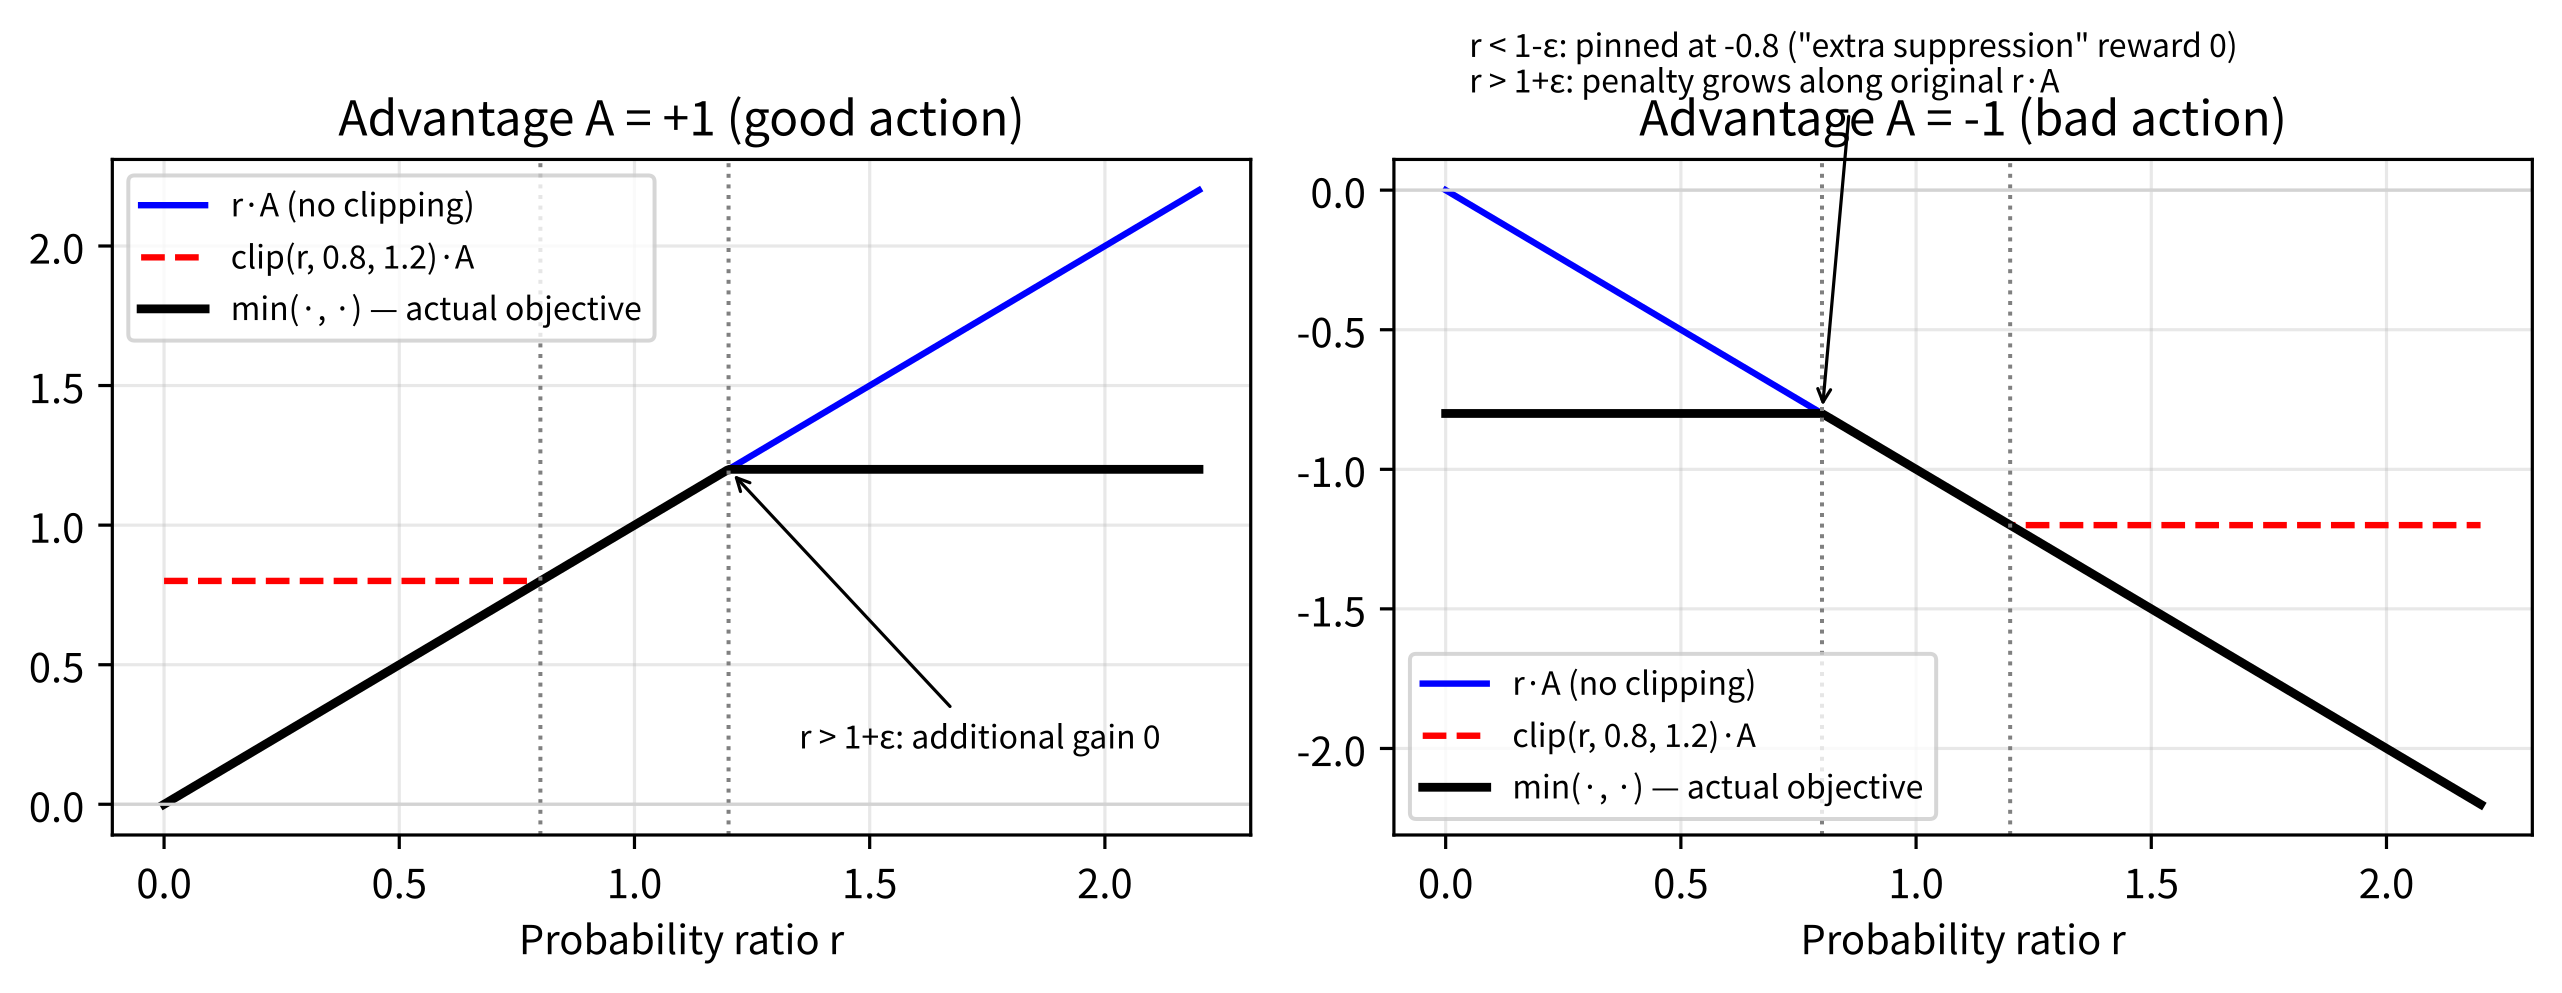
\includegraphics[width=\linewidth]{ch11_2_ppo_clip_loss.png}
      {\footnotesize 한 샘플분, $\epsilon=0.2$, $r_t$ 를 0$\sim$2.2
     까지. 파랑 실선 = $r_tA_t$, 검정 = 실제 목적함수, 빨강 점선 =
      $\mathrm{clip}(r_t,0.8,1.2)\,A_t$, 회색 세로점선 = 클립
      경계.}
    \end{column}
    \begin{column}{0.40\textwidth}
      {\small
      \kb{왼쪽 $A=+1$(좋은 행동)}
      \begin{itemize}
        \item $r_t\in[0.8,1.2]$ 안: 검은 곡선 = 파랑 실선
          (원래 중요도 목적함수 그대로).
        \item $r_t>1.2$ 순간: \textbf{수평으로 꺾임} —
          ``좋은 행동을 추가로 더 밀어주는 것''의 보상이 0.
      \end{itemize}
      \kb{오른쪽 $A=-1$(나쁜 행동)}
      \begin{itemize}
        \item $r_t<0.8$: 목적함수가 \textbf{−0.8로 고정} —
          ``나쁜 행동을 조금 더 덜 선호하게 하는 것''의 추가
          보상 0.
        \item $r_t>1.2$ (나쁜 것을 더 선호하는 방향): 벌금은
          \textbf{상한 없이} 계속 커진다.
      \end{itemize}}
    \end{column}
  \end{columns}
\end{frame}

\begin{frame}{클리핑의 비대칭: 상한은 ``개선 방향''에만}
  \small
  두 패널을 함께 읽으면 min의 역할이 정확히 보인다:
  \begin{itemize}
    \item \kb{범위 안}($r_t\in[0.8,1.2]$): 원래 중요도 목적함수
      $r_tA_t$ 그대로 — $r_t=1$ 근처(데이터 수집 직후)에서는
      REINFORCE 계열 그래디언트와 본질적으로 같은 방향.
    \item \kb{범위 밖, 개선 방향}: ``좋은 것을 더 밀어주는 것''과
      ``나쁜 것을 더 억제하는 것''의 \textbf{추가 이득이 0}
      (검은 곡선 수평).
    \item \kb{범위 밖, 악화 방향}: ``나쁜 것을 더 밀어올리는 것''
     에는 \textbf{상한이 없다}.
  \end{itemize}
  \vskip0.5em
  \begin{block}{미분으로 보면 더 명확}
    목적함수가 수평인 구간에서는 $r_t$ 에 대한 기울기가 정확히 0 —
    ``추가 이득이 0''은 문자 그대로 ``이 방향으로는 그만''.
    \kb{min이 ``비관적(더 작은)쪽''을 고르기 때문에} 자연스럽게
    생기는 비대칭.
  \end{block}
\end{frame}

\begin{frame}{손으로 계산해 보기 — $\epsilon=0.2$}
  \small
  \begin{tabular}{@{}llll@{}}
    \toprule
    & & $A_t=+1$ (좋은 행동) & $A_t=-1$ (나쁜 행동) \\
    \midrule
    $r_t=0.5$ &
      clip 안 됨 (범위 안) & $\min(0.5,\,0.5)=\mathbf{0.5}$ &
      $\min(-0.5,\,-0.8)=\mathbf{-0.8}$ (clip 쪽 채택) \\
    $r_t=1.5$ &
      clip 1.2 이 됨 & $\min(1.5,\,1.2)=\mathbf{1.2}$ (잘림) &
      $\min(-1.5,\,-1.2)=\mathbf{-1.5}$ (원래 곡선 채택) \\
    \bottomrule
  \end{tabular}
  \vskip0.7em
  \begin{itemize}
    \item $A_t=+1,\, r_t=1.5$: 초과분 이득(0.3)은 인정하지 않음 —
      ``좋은 행동을 더'' 방향에서 멈춤.
    \item $A_t=-1,\, r_t=1.5$: \textbf{clip 안 한 쪽}이 더 작아서
      그대로 — ``나쁜 것을 더 선호하게 만드는'' 방향에는 클립이
      발동하지 않고 벌금이 계속 커진다.
    \item $A_t=-1,\, r_t=0.5$: clip 쪽($-0.8$)이 더 작아서 채택 —
      ``나쁜 것을 덜 선호하게 만드는'' 방향은 $-0.8$
      $(=(1-\epsilon)A)$ 에서 멈춘다.
  \end{itemize}
  \begin{block}{핵심}
    min은 ``클립 안 한 값''을 무조건 고르는 것이 아니라,
    \kb{항상 두 값 중 더 작은(비관적인) 쪽}을 고르는 기계적
    장치. $A_t$ 의 부호와 $r_t$ 의 크기에 따라 ``어디서
    멈추는가''가 달라진다.
  \end{block}
\end{frame}

\begin{frame}{자주 하는 실수 — min/max, 절대 확률}
  \begin{itemize}
    \item \kb{실수 1: max를 쓰는 것.} 목적함수를 \textit{최대화}
      하므로 min(비관적 쪽)을 써야 하는데, max를 쓰면 역할이
      뒤집힌다 — 좋은 행동($A_t>0$)에서는 $r_t>1+\epsilon$ 일 때
      max가 \textbf{클립 안 한 쪽} $r_tA_t$ 를 계속 고르므로 좋은
      행동을 밀어주는 것에 상한이 \textbf{사라진다}(클리핑이
      막으려던 폭주가 그대로 남는 방향).
    \item \kb{실수 2: 클립 경계를 ``절대 확률 0.8$\sim$1.2''로
      오해.} 클립 대상은 \textbf{비} $r_t$ 이지 행동이나 확률
      자체가 아니다.
  \end{itemize}
  \vskip0.5em
  \begin{block}{올바른 뜻}
    ``\kb{옛 정책 대비} 이 행동의 상대적 선호가 20\% 이내여야
    한다'' — 옛 정책이 확률 0.01을 준 행동에 대해 새 정책이
    0.012까지, 0.5를 준 행동에 대해 0.6까지 올릴 수 있다.
    같은 ``20\%''라도 절대값으로 바뀌면 극단적 확률의 행동이
    영원히 갱신되지 못한다.
  \end{block}
\end{frame}

\begin{frame}{PPO 원 논문의 서브게이트 함수 (Figure 1)}
  \begin{columns}[T]
    \begin{column}{0.62\textwidth}
      \centering
      
\includegraphics[width=\linewidth]{ref_ppo.png}
    \end{column}
    \begin{column}{0.36\textwidth}
      {\small
      서브게이트 함수 $L^{\mathrm{CLIP}}$ 의 한 항(단일
      timestep)을 확률비 $r$ 의 함수로 그린 그래프.
      \\[0.8em]
      \kb{좌}: 이익이 양수 ($A>0$) — $r>1+\epsilon$ 에서 수평.
      \\[0.6em]
      \kb{우}: 이익이 음수 ($A<0$) — $r<1-\epsilon$ 에서 수평,
      $r>1+\epsilon$ 쪽은 계속 하강.
      \\[0.8em]
      min이 만드는 ``모서리''가 원 논문에서도 동일한 형태.
      }
    \end{column}
  \end{columns}
\end{frame}

\begin{frame}{PPO의 전체 목적함수 — 세 항}
  \small
  실전 PPO는 Actor-Critic 구조(10.3절)이므로, $L^{\mathrm{CLIP}}$
  은 \textbf{정책(Actor) 부분}만. 실제 미니배치 갱신:
  \[
  L(\theta) = \underbrace{\mathbb{E}_t\Big[\min\Big(r_tA_t,\;
  \mathrm{clip}(r_t,1-\epsilon,1+\epsilon)A_t\Big)\Big]}
  _{\text{정책 손실(최대화)}}
  \underbrace{-\,c_v\,\mathbb{E}_t\big[(V_\theta(s_t)-\hat{R}_t)^2\big]}
  _{\text{Critic 손실(최소화)}}
  \underbrace{+\,c_e\,\mathbb{E}_t\big[\mathcal{H}(\pi_\theta
  (\cdot\mid s_t))\big]}_{\text{엔트로피 보너스(탐험 유지)}}
  \]
  \begin{itemize}
    \item $V_\theta$ = 10.3절 Critic, $\hat{R}_t$ = Critic
      업데이트 목표값 (실습: GAE로 계산한 어드밴티지 $+V$).
    \item $c_v,\,c_e$ = 손실 스케일 정규화 상수 (실습: 0.5, 0.01).
    \item 엔트로피 항 = Chapter 5.2의 $\epsilon$-greedy의
      \textbf{연속 버전}.
  \end{itemize}
\end{frame}

\begin{frame}{엔트로피 보너스: $\log\sigma$ 를 잡아당기는 브레이크}
  \kq{왜 엔트로피 보너스를 넣으면 탐험이 유지되는가?}
  \vskip0.5em
  \begin{itemize}
    \item 엔트로피 = 분포가 얼마나 퍼져 있는지의 척도 — Chapter 2
      UCB와 같은 ``탐험 유인''의 연속.
    \item \kb{정규분포 정책에서는 엔트로피가 $\log\sigma$ 에
      비례} — 이 항은 \textbf{표준편차를 줄이는 경향을 계속 반대
      방향으로 잡아당기는 항}.
    \item 정책이 ``이 토크가 정답이야''라고 확신을 가지는 속도를
      조절하는 \kb{브레이크} — 너무 빨리 \textbf{단정적으로} 하나에
      수렴해서(탐험이 끝나버려서) 로컬 최적에 끼는 걸 늦춘다.
  \end{itemize}
  \vskip0.5em
  \begin{block}{역사: PPO-1과 PPO-2}
    PPO 논문(Schulman, Moritz et al., 2017)에는 알고리즘이
    \textbf{둘} 들어 있다. \kb{PPO-1}: 경사 ascent 스텝 자체를
    ``KL 제약 이해를 확인하며'' 잘게 쪼개는 방식 (TRPO line
    search의 단순형). \kb{PPO-2}: 클리핑만 한 버전 — 논문 공개 후
    ``더 단순하고 실전에서 거의 차이가 없거나 오히려 낫다''는
    말이 빠르게 퍼져 \textbf{클리핑 버전(PPO-2)이 표준}.
    ML 역사에서 드문 경우: ``더 단순한'' 두 번째 버전이
    커뮤니티에 의해 선택됨.
  \end{block}
\end{frame}

\begin{frame}[fragile]{실습: Pendulum에서 PPO — 가우시안 정책}
  Pendulum-v1: 진자를 세워서 유지하는 고전 연속 제어 과제, 행동은
  \textbf{$-2\sim+2$Nm의 토크 하나}. 연속 행동공간에서는 정책이
  정규분포의 평균·표준편차를 출력.
  \begin{lstlisting}
class GaussianPolicy(nn.Module):
    def __init__(self, state_dim, act_dim):
        super().__init__()
        self.net = nn.Sequential(nn.Linear(state_dim,64), nn.Tanh(),
                                 nn.Linear(64,64), nn.Tanh())
        self.mu = nn.Linear(64, act_dim)
        self.log_std = nn.Parameter(torch.zeros(act_dim) - 0.5)  # 학습 가능한 표준편차
    def forward(self, x):
        h = self.net(x)
        mu = torch.tanh(self.mu(h)) * act_high   # 행동 범위에 맞게 스케일
        std = torch.exp(self.log_std)
        return mu, std
  \end{lstlisting}
  \vskip0.2em
  {\footnotesize 행동 샘플링: $\mathrm{dist}=\mathrm{Normal}
  (\mu,\mathrm{std})$; $\ a=\mathrm{dist.sample()}$;
  $\ \log p=\mathrm{dist.log\_prob}(a).\mathrm{sum()}$. GAE로
  advantage 계산 $\to$ 4 에폭 미니배치 재사용 $\to$
  ppo\_clip\_loss로 정책 갱신.}
\end{frame}

\begin{frame}{연속 공간의 확률비 — 가우시안 로그가능도 미분}
  이산(softmax)에서는 $\pi_\theta(a\mid s)$ 가 단일 확률 값,
  연속에서는 행동 $a$ 가 연속 변수이므로 $\pi_\theta(a\mid s)$ 는
  \textbf{정규분포 $\mathcal{N}(\mu_\theta(s),\sigma_\theta^2)$ 의
  가능성(density)}.
  \small
  \[
  \log\pi_\theta(a\mid s) = -\frac{1}{2}\Big(\frac{a-\mu_\theta(s)}
  {\sigma_\theta}\Big)^{\!2} - \log\sigma_\theta + \mathrm{const}
  \]
  \[
  \nabla_\theta\log\pi_\theta(a\mid s)
  = \underbrace{\frac{a-\mu_\theta(s)}{\sigma_\theta^2}\,
  \nabla_\theta\mu_\theta(s)}_{\mu\ \mathrm{항}}
  + \underbrace{\frac{(a-\mu_\theta(s))^2-\sigma_\theta^2}
  {\sigma_\theta^3}\,\nabla_\theta\sigma_\theta}_{\sigma\ \mathrm{항}}
  \]
  {\footnotesize 정규분포 로그가능도의 $-\log\sigma$ 정규화 항이
  없으면 $\sigma$ 미분식에 $-1/\sigma$ 가 빠져 \textbf{틀어진다} —
  빼먹기 쉬운 부분.}
\end{frame}

\begin{frame}{$\mu$ 항이 주인공, $\sigma$ 항은 보조 변수}
  \begin{itemize}
    \item 핵심 구조는 \kb{Policy Gradient Theorem의 one-vs-rest
      일반화}. 10.2절 softmax 그래디언트
      $[(1-p_a)s,\ -p_as]$ 의 ``고른 행동 확률 올리고, 나머지는
      내린다''가, 정규분포에서는 \kb{``고른 행동 쪽으로 평균을
      이동시킨다''}로 바뀜.
    \item \kb{$\mu$ 항}: 부호는 $a-\mu$ 의 부호로 정해짐.
      $A_t>0$ 이면 고른 행동 쪽으로 평균이 당겨지고, $A_t<0$
      이면 반대로 밀려남 — softmax의 ``고른 행동을 올린다''가
      정확히 이 $\mu$ 항.
    \item \kb{$\sigma$ 항}: 부호가 $(a-\mu)^2-\sigma^2$ 로 정해져
      까다로움.
      \begin{itemize}
        \item $|a-\mu|>\sigma$ (``의도하지 않은 극단적 행동'')
          $\to$ $\sigma$ \textbf{줄이는} 방향.
        \item $\sigma$ 이내(보통의 경우) $\to$ $\sigma$
          \textbf{늘리는} 방향.
      \end{itemize}
  \end{itemize}
  \begin{block}{기억하면 충분한 큰 그림}
    \kb{$\mu$ 가 주된 학습 대상이고, $\sigma$ 는 $A_t$ 의 부호와
    엔트로피 보너스 사이에 놓인 보조 변수}.
  \end{block}
\end{frame}

\begin{frame}[fragile]{전체 알고리즘 루프}
  \texttt{GaussianPolicy} 만으로는 PPO가 아니다 —
  ``데이터를 모은 뒤 여러 번 재사용하면서 클리핑으로 업데이트를
  제한한다''는 절차가 PPO의 본체.
  \begin{lstlisting}
for iteration in range(N_ITER):          # 보통 수백 회
    # (1) 현재 정책으로 STEPS 스텝 상호작용: (s,a,r,s') 수집
    #     + 각 스텝의 logp_old = log pi_old(a|s), V_old(s) 저장
    # (2) GAE로 각 스텝의 A_t, 리턴 목표 R_t 계산 (11.3절)
    #     A_t = A_t - mean / std 로 정규화
    for epoch in range(N_EPOCH):         # (3) 같은 데이터 4~10 에폭 재사용
        for minibatch in shuffle_split(collected, MB_SIZE):
            mu, std, v = actor_critic(s_batch)
            logp_new = Normal(mu, std).log_prob(a_batch).sum()
            ratio = exp(logp_new - logp_old)    # <-- 11.1절의 r_t
            loss = -min(ratio*A, clip(ratio,1-eps,1+eps)*A).mean() \
                   + 0.5*((v - R_batch)**2).mean() \
                   - 0.01*Normal(mu, std).entropy().sum()
            optimizer.step()
    # (4) 이 iteration에 모은 데이터 버림 -> (1)로
  \end{lstlisting}
\end{frame}

\begin{frame}{세 가지 ``왜''}
  \small
  \begin{itemize}
    \item \kb{왜 (1)에서 \texttt{logp\_old}를 저장하는가?}
      $r_t=\pi_\theta/\pi_{\theta_{\mathrm{old}}}$ 의 분모는
      \textbf{데이터를 모았을 때의} 정책 — 그 당시 로그가능도를
      저장해두고, (3)에서 현재 정책의 로그가능도를 계산해 비를
      만든다. 저장하지 않으면 $\theta$ 가 이미 바뀐 뒤 재계산해
      비가 1이 되는 시점이 ``데이터 수집 시점''이 아니라
      ``갱신 시점''이 된다.
    \item \kb{왜 (3)를 여러 에폭 돌리는가?} Chapter 9.4 재현 버퍼는
      데이터를 \textit{영원히} 저장, PPO는 \textbf{몇 에폭만}
      쓰고 버림 — 클리핑이 ``몇 에폭 재사용''이라는 제한 안에서만
      안정성을 보장.
    \item \kb{왜 (4)에서 버리는가?} on-policy 가정(데이터를 모은
      정책 $\approx$ 현재 정책)이 에폭을 거듭할수록 깨져, $r_t$ 가
      클립 범위를 벗어나는 샘플이 많아지기 때문.
  \end{itemize}
\end{frame}

\begin{frame}{Pendulum 학습 결과 (300 반복 $\times$ 400 스텝)}
  \begin{columns}[T]
    \begin{column}{0.56\textwidth}
      \centering
      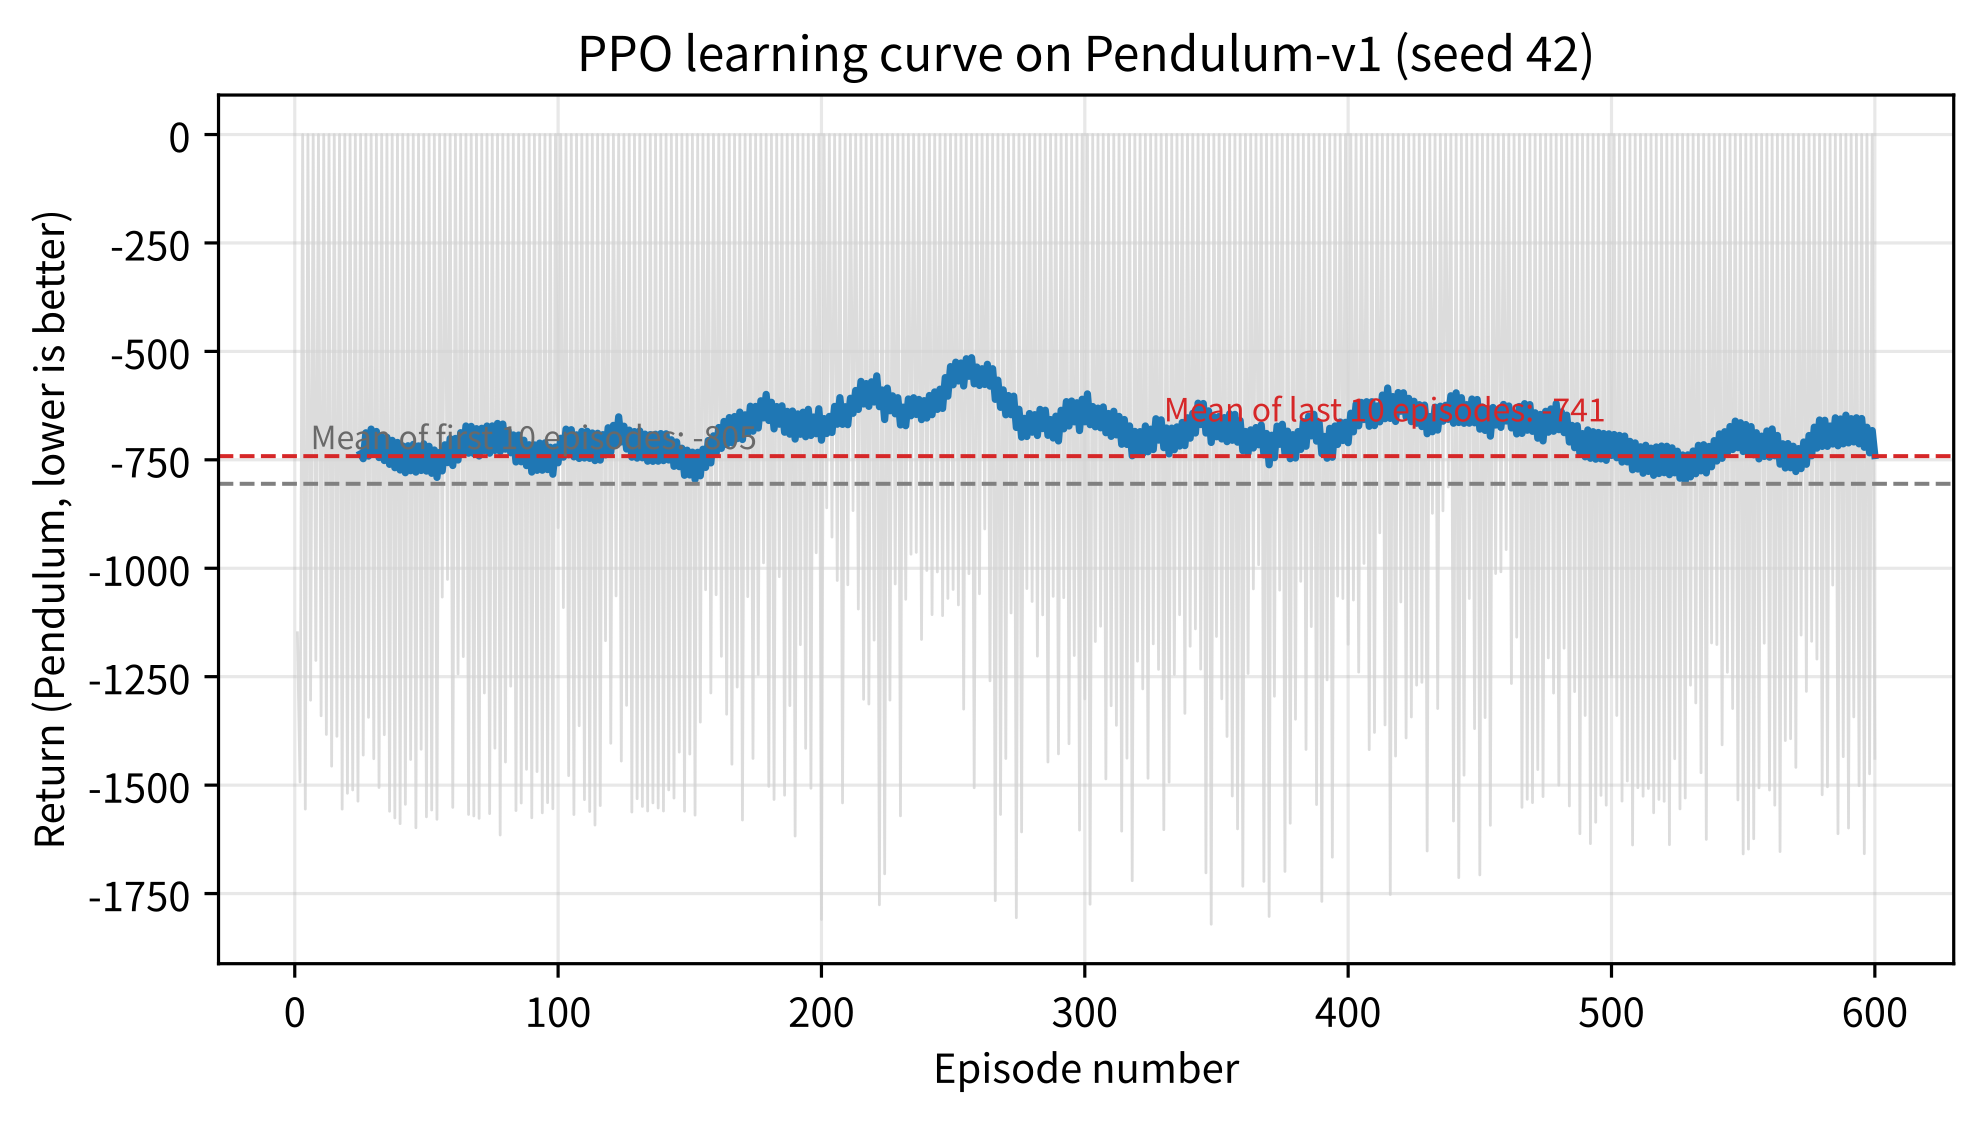
\includegraphics[width=\linewidth]{ch11_2_ppo_pendulum_curve.png}
      {\footnotesize 시드 42, 총 12만 스텝. 연회색 = 에피소드별
      리턴(항상 음수, 0에 가까울수록 좋음), 파랑 실선 = 25에피소드
      이동평균.}
    \end{column}
    \begin{column}{0.42\textwidth}
      {\small
      \begin{tabular}{@{}lr@{}}
        \toprule
        처음 10 에피소드 평균 & $-805.3$ \\
        마지막 10 에피소드 평균 & $-742.3$ \\
        \bottomrule
      \end{tabular}
      \vskip0.5em
      \begin{itemize}
        \item 약 \textbf{8\%} 개선, 여전히 절댓값이 크고 학습
          곡선도 매끄럽지 않음 (중간 지점에서 오히려 나빠지는
          구간도 있었음).
        \item 구현 오류가 아니라, Pendulum 같은 연속 제어는
          완전 수렴에 \textbf{수십만$\sim$수백만 스텝}이 필요
          — 정직한 결과.
        \item DQN(CartPole, 300에피소드 만에 상당한 개선, 9.3절)
          과 비교: 연속 제어가 이산보다 \textbf{더 오래} 걸림.
      \end{itemize}}
    \end{column}
  \end{columns}
\end{frame}

\begin{frame}{곡선의 ``모양''에서 두 가지를 읽기}
  \begin{itemize}
    \item \kb{첫째 — 개별 에피소드의 변동폭이 크다.}
      \small
      Pendulum 리턴은 에피소드 초반에 쓰러지면 $-1800$ 근처
      (이번 실행 최소 $-1820.6$), 진자를 거의 수직으로 버티면
      0 근처(최대 $0.0$ — upright 평형점 근처에 오래 머문 뜻)로
      넓게 퍼짐. 10.2절 REINFORCE에서 배운
      \kb{``단일 에피소드 리턴의 분산이 크다''}는 문제와
      \textbf{정확히 같은 본질} — PPO는 GAE(11.3)와 어드밴티지
      정규화로 이 분산을 \textit{그래디언트} 차원에서 줄이되,
      \textit{에피소드 리턴 자체}의 분산은 줄일 수 없다.
    \item \kb{둘째 — 이동평균이 완만하게만 올라간다.}
      \small
      ``학습이 안 된다''기보다 \textbf{12만 스텝이 이 과제에겐
      부족하다} — Ch.\,13$\sim$14 로봇 시뮬레이션에서 보통
      수백만 스텝을 계획하는 이유. (다른 seed에서는 마지막 10
      에피소드 평균이 $\pm100\sim200$ 차이, ``완만한 상승''은
      seed마다 안정적.)
  \end{itemize}
\end{frame}

\begin{frame}{자주 하는 실수 — $\theta_{\mathrm{old}}$ 를 갱신
스텝마다 다시 계산하기}
  \begin{itemize}
    \item (2)$(\sim)$(3) 구간에서 ``데이터를 모았을 때의 정책''
      이 아니라 \textbf{``지금 이 갱신 스텝의 정책''}으로 $r_t$
      의 분모를 계산하면,
    \item $r_t$ 가 \textbf{항상 1 근처}(갱신 전의 현재 정책 대비
      갱신 후의 현재 정책)로 압박되어 \textbf{클리핑이 거의
      발동하지 않는다} —
    \item 결과적으로 PPO가 \kb{``클리핑 없는 REINFORCE''로
      전락}.
  \end{itemize}
  \vskip0.6em
  \begin{block}{11.1절의 핵심을 기억하자}
    $r_t$ 는 \textbf{옛 정책}(데이터 수집 시점)과 \textbf{새
    정책}(갱신 시점)의 비이며, 분모의 ``옛''은
    \kb{데이터 수집 시점}이지 \textit{갱신 직전}이 아니다.
    실습 코드의 \texttt{logp\_old}를 (1) 구간에서 저장해두는
    이유가 바로 이것.
  \end{block}
\end{frame}

\begin{frame}{자주 묻는 질문 — 구현 선택들}
  \small
  \begin{itemize}
    \item \kb{Q. \texttt{log\_std}를 왜 상태와 무관한 파라미터로?}
      구현 단순화 — ``탐험 정도는 학습이 진행되며 전역적으로
      줄어든다''는 가정 하나로 충분. (상태별 탐험을 원하면 신경망
      출력으로 만들 수 있음.)
    \item \kb{Q. 왜 매 반복마다 데이터를 새로 모으나요?}
      PPO는 on-policy의 연장선 — 클리핑은 ``$r_t$ 가 1에서 크게
      벗어나지 않는다''는 전제로 설계. 오래된 데이터(정책이 많이
      바뀜)는 애초에 $r_t$ 가 클리핑 범위를 크게 벗어나 거의
      기여 못 함. Ch.\,9 경험재현(오래된 데이터 계속 재사용)과
      \textbf{정반대}의 전략.
    \item \kb{Q. $\texttt{torch.exp}(\texttt{log\_std})$ 의 이유는?}
      $\sigma>0$ 제약(표준편차는 양수)을 \textbf{파라미터 공간
      자체에서} 강제 — $\log\sigma$ 는 $(-\infty,+\infty)$
      에서 자유롭게 움직여도 $\exp$ 후에는 항상 양수.
      Ch.\,5 softmax가 logit 공간을 쓰는 것과 동일한 ``제약을
      파라미터 공간 밖으로 밀어낸다'' 전략.
  \end{itemize}
\end{frame}

\begin{frame}{자주 묻는 질문 — $\epsilon$ 튜닝과 연속 vs 이산}
  \small
  \begin{itemize}
    \item \kb{Q. $\epsilon$ 을 0.05 또는 0.5로?}
      \begin{itemize}
        \item 작으면 클립 구간 좁아져 한 번에 이동할 수 있는
          거리 감소 — \textbf{안정성은 올라가지만 학습 느려짐}.
        \item 크면 클립이 거의 발동하지 않아 사실상
          \textbf{REINFORCE로 수렴}(더 공격적).
        \item 실제 튜닝: 0.1$\sim$0.3 사이 탐색, 0.2는
          ``안정성 vs 속도'' 균형점의 경험적 기본값.
          ($\epsilon$ 과 GAE의 $\lambda$ 는 독립적
          하이퍼파라미터이나 함께 안정성에 영향 — 11.3 FAQ.)
      \end{itemize}
    \item \kb{Q. Pendulum이 DQN(CartPole)보다 느린 이유
      (연속 vs 이산)?}
      \begin{itemize}
        \item 이산: 최적점이 확률 벡터의 \textbf{꼭짓점}
          (예: $[1,0]$) — softmax가 꼭짓점 \textit{근처}까지만
          밀어주면 됨.
        \item 연속: 상태마다 ``맞는 토크''가 연속 값 —
          $\mu_\theta(s)$ 가 \textbf{연속 매개변수 곡면 전체}를
          상태별로 적절히 맞춰야 하고 $\sigma_\theta$ 도 함께
          학습, 탐색할 파라미터 공간이 무한대. ``근처까지''가
          아니라 매 상태별 ``적절한 값''에 접근해야 함 —
          연속 제어가 근본적으로 어려운 점.
      \end{itemize}
  \end{itemize}
\end{frame}

\begin{frame}{11.2절 요약}
  \begin{itemize}
    \item PPO는 TRPO의 ``신뢰 영역'' 아이디어를, 2차 미분
      최적화 대신 \kb{목적함수 안의 min(클리핑) 한 줄}로 구현.
    \item min이 만드는 모서리: \textbf{개선 방향(좋은 것을 더,
      나쁜 것을 덜)의 과도한 이동에만} 상한, 악화 방향에는
      없음 — ``비관적 쪽을 고르는'' min의 비대칭.
    \item 전체 목적함수 = \kb{정책 손실($L^{\mathrm{CLIP}}$) +
      Critic 손실 $-$ 엔트로피 보너스} — 엔트로피 항이
      $\log\sigma$ 를 잡아당겨 탐험을 유지.
    \item Pendulum 실습: 연속 제어는 이산 제어보다 느리지만, 그
      느림은 구현의 결함이 아니라 \textbf{연속 행동공간의 탐색
      체적}이라는 본질적 요인.
  \end{itemize}
  \vskip0.5em
  \begin{block}{지금까지의 PPO}
    ``구현하기 쉽고, 실전에서 잘 작동하는'' 알고리즘 — 지금 가장
    널리 쓰이는 정책기반 알고리즘.
  \end{block}
\end{frame}

\section{11.3 GAE와 PPO가 표준이 된 이유}

\begin{frame}{위치: 골격만으로는 실전에 못 쓴다}
  11.2절까지 PPO의 골격(확률비 $\to$ 클리핑 $\to$ 미니배치
  재사용)을 세웠지만, 골격만으로는 실전에 못 쓴다 — 11.2절
  실습의 학습 곡선은 매끄럽지 않았고, Pendulum은 30만 스텝에도
  $-1092$ 에서 멈췄다.
  \vskip0.6em
  \begin{itemize}
    \item ``PPO가 잘 동작한다''는 평판을 만들어준
      \textbf{마지막 두 조각} = \kb{GAE}(Generalized Advantage
      Estimation, 2016) + \kb{엔트로피 보너스}.
    \item 이번 절: 그 둘을 배우고, 왜 PPO가
      (1) 이론적으로는 TRPO(2015)에 못 미치고
      (2) 구현은 \textbf{100배 단순}한데도 TRPO를 사실상
      완전히 밀어내버렸는지 — ``표준이 된 이유''를 정리.
    \item 마지막으로 ``PPO를 돌린다''는 말이 실제로 어떤 코드
      묶음을 의미하는지 실전 스택 전체를 훑음.
  \end{itemize}
\end{frame}

\begin{frame}{GAE 원 논문의 학습 곡선 (Figure 1)}
  \begin{columns}[T]
    \begin{column}{0.60\textwidth}
      \centering
      
\includegraphics[width=\linewidth]{ref_gae.png}
    \end{column}
    \begin{column}{0.38\textwidth}
      {\small
      3D 워커 환경 학습 곡선. \kb{PPO+GAE} (청색)가 DDPG /
      TRPO / SAC 대비 \textbf{더 적은 반복 횟수로 높은 보상}을
      달성.
      \\[0.8em]
      GAE가 ``평판''의 절반을 만들었다 — 11.2절의 골격만
     으로는 이 곡선이 나오지 않는다.
      }
    \end{column}
  \end{columns}
\end{frame}

\begin{frame}{GAE: TD와 MC 사이를 $\lambda$ 다이얼로}
  10.3절의 어드밴티지 $A_t=G_t-V(s_t)$ 는 실제 리턴 $G_t$ 를
  그대로 쓰므로 여전히 \textbf{분산이 크다}.
  \vskip0.5em
  \kb{GAE} = Chapter 7의 n-step/적격흔적 아이디어를
  \textbf{어드밴티지 추정}에 적용 — 여러 $n$-step 어드밴티지를
  $\lambda$ 로 가중평균, 분산은 낮추되 편향은 적당히만 감수:
  \[
  A_t^{\mathrm{GAE}} = \sum_{k=0}^{\infty}
  (\gamma\lambda)^{k}\,\delta_{t+k},
  \qquad
  \delta_t = r_t + \gamma V(s_{t+1}) - V(s_t)
  \]
  \begin{itemize}
    \item $\delta_t$ 는 6.1절의 \kb{TD 오차} 그 자체 — GAE는
      ``\textbf{여러 시점의 TD 오차를 적격흔적처럼 지수적으로
      가중합}해서 하나의 어드밴티지 추정치를 만든다''.
    \item $\lambda=0$: \kb{TD(0) 기반} (분산 작고 편향 큼).
      \; $\lambda=1$: \kb{몬테카를로 기반} (편향 없고 분산 큼).
    \item 7.2절의 다이얼이 여기서도 그대로 — 실전 PPO는
      \textbf{거의 항상} GAE로 계산한 $A_t$ 를 사용
      (11.2절 \texttt{compute\_gae} 가 바로 이 식).
  \end{itemize}
\end{frame}

\begin{frame}{n-step 어드밴티지와 GAE의 관계}
  \small
  $n$-step 어드밴티지를 따로 정의:
  \[
  A_t^{(n)} := G_t^{(n)} - V(s_t) = \sum_{k=0}^{n-1}
  \gamma^{k}\,\delta_{t+k}
  \]
  \begin{itemize}
    \item \kb{직접 확인할 것}: 두 식은 정확히 같다 — 좌변을
      전개하면 실제 보상 $r_t+\gamma r_{t+1}+\cdots$ 가 나오고,
      우변의 각 $\delta$ 를 정의대로 전개하면 같은 보상들이
      $\gamma^k$ 로 할인되어 합쳐지며, \textbf{가운데의 $V$ 들이
      연속적으로 상쇄}(telescoping:
      $\gamma V(s_{t+1})-\gamma V(s_{t+1})$ 등).
    \item $n=1$ 이면 $A_t^{(1)}=\delta_t$, 에피소드 길이보다
      큰 $n$ 이면 $A_t^{(n)}=G_t-V(s_t)$ (10.3절 원래 정의).
  \end{itemize}
  \vskip0.5em
  \begin{block}{정리 (수식은 한 줄)}
    \[
    A_t^{\mathrm{GAE}} = (1-\lambda)\sum_{n=1}^{\infty}
    \lambda^{\,n-1}\,A_t^{(n)}
    \]
    \kb{$A_t^{\mathrm{GAE}}$ 는 $n$-step 추정치들의 지수적
    가중평균}.
  \end{block}
  \vskip0.5em
  \begin{enumerate}
    \item 각 $A_t^{(n)}$ 을 위 telescoping 식으로 바꾸면, 같은
      $\delta_{t+k}$ 를 만드는 모든 $n$ ($n>k$, 즉
      $n=k+1,k+2,\ldots$)에서 해당 $\delta$ 가 $\gamma^k$
      계수로 한 번씩 등장.
    \item $(1-\lambda)\sum_{n=k+1}^{\infty}\lambda^{n-1}\gamma^k
      = (\gamma\lambda)^k$ — 지수급수의 꼬리를 정리하면
      바로 무한합 정의가 나옴.
  \end{enumerate}
  \vskip0.6em
  \begin{block}{7.2절과의 연결}
    $\lambda$ 는 ``어떤 $n$-step 추정치를 얼마나 신뢰하는지''를
    결정하는 \kb{가중 분포} $\propto\lambda^{n-1}$.
    7.2절에서 적격흔적이 ``n 하나를 고르는 것''을
    ``\textbf{모든 n의 가중분포}로 승화''시켰던 것과
    \textbf{같은 승화} — GAE를 ``어드밴티지에 적용한
    적격흔적''이라 부르는 이유.
  \end{block}
\end{frame}

\begin{frame}{손으로 계산: 3스텝 에피소드의 TD 오차}
  에피소드 3스텝: $s_0\to s_1\to s_2\to s_3$ ($s_3$ 터미널),
  $\gamma=0.9$, critic의 값 $V=[2.0,\,1.4,\,0.6,\,0]$, 보상
  $r=[1,\,1,\,0]$.
  \vskip0.6em
  \kb{TD 오차} $\delta_t = r_t + \gamma V(s_{t+1}) - V(s_t)$:
  \small
  \begin{tabular}{@{}lll@{}}
    \toprule
    스텝 & 계산 & $\delta$ \\
    \midrule
    $t=0$ & $1 + 0.9\times1.4 - 2.0$ & $+0.26$ \\
    $t=1$ & $1 + 0.9\times0.6 - 1.4$ & $+0.14$ \\
    $t=2$ & $0 + 0.9\times0 - 0.6$ & $-0.60$ \\
    \bottomrule
  \end{tabular}
  \vskip0.8em
  첫 스텝 $s_0$ 의 GAE를 $\lambda$ 별로 계산 — 각 항 가중계수
  $(1,\ \gamma\lambda,\ \gamma^2\lambda^2)$:
\end{frame}

\begin{frame}{$\lambda$ 를 바꾸면 부호까지 바뀐다}
  \small
  \begin{tabular}{@{}lcll@{}}
    \toprule
    $\lambda$ & 가중계수 $(1,\gamma\lambda,\gamma^2\lambda^2)$
      & $A_0^{\mathrm{GAE}}$ & 읽기 \\
    \midrule
    0.0 & $(1,\ 0,\ 0)$ & $0.26$ & $\delta_0$ 하나만 — ``1스텝만
      보고'' (TD(0)) \\
    0.5 & $(1,\ 0.45,\ 0.2025)$ &
      $0.26+0.45(0.14)+0.2025(-0.60)=+0.20$ & 중간 — 세 항 다
      포함 \\
    0.95 & $(1,\ 0.855,\ 0.731)$ & $-0.059$ & 거의 MC \\
    1.0 & $(1,\ 0.9,\ 0.81)$ &
      $G_0-V(s_0)=1.9-2.0=-0.10$ & 전체 리턴 기준 (MC) \\
    \bottomrule
  \end{tabular}
  \vskip0.8em
  \begin{itemize}
    \item \textbf{같은 데이터}($\delta_0,\delta_1,\delta_2$)인데
      $\lambda$ 만 바꾸면 $+0.26$(좋았다)에서 $-0.10$(나빴다)까지
      \kb{부호까지} 바뀜.
    \item $\lambda$ 가 ``\kb{신뢰하는 지평선의 길이}''이라는
      뜻: 짧은 지평선($\lambda\approx0$)은 ``지금 당장의 TD
      오차만 믿는다''(분산 적음, $V$ 의 오차가 편향으로),
      긴 지평선($\lambda=1$)은 ``에피소드 전체의 실제 리턴을
      믿는다''(편향 없음, 리턴의 흔들림이 분산으로).
    \item 실전 기본값 $\lambda=0.95$ = ``긴 지평선에 거의
      의존하되, 가장 먼 꼬리만 5\% 정도로 얕은 신뢰''의 절충.
  \end{itemize}
\end{frame}

\begin{frame}{편향-분산 U자 — 이론이 아니라 실험}
  \begin{columns}[T]
    \begin{column}{0.58\textwidth}
      \centering
      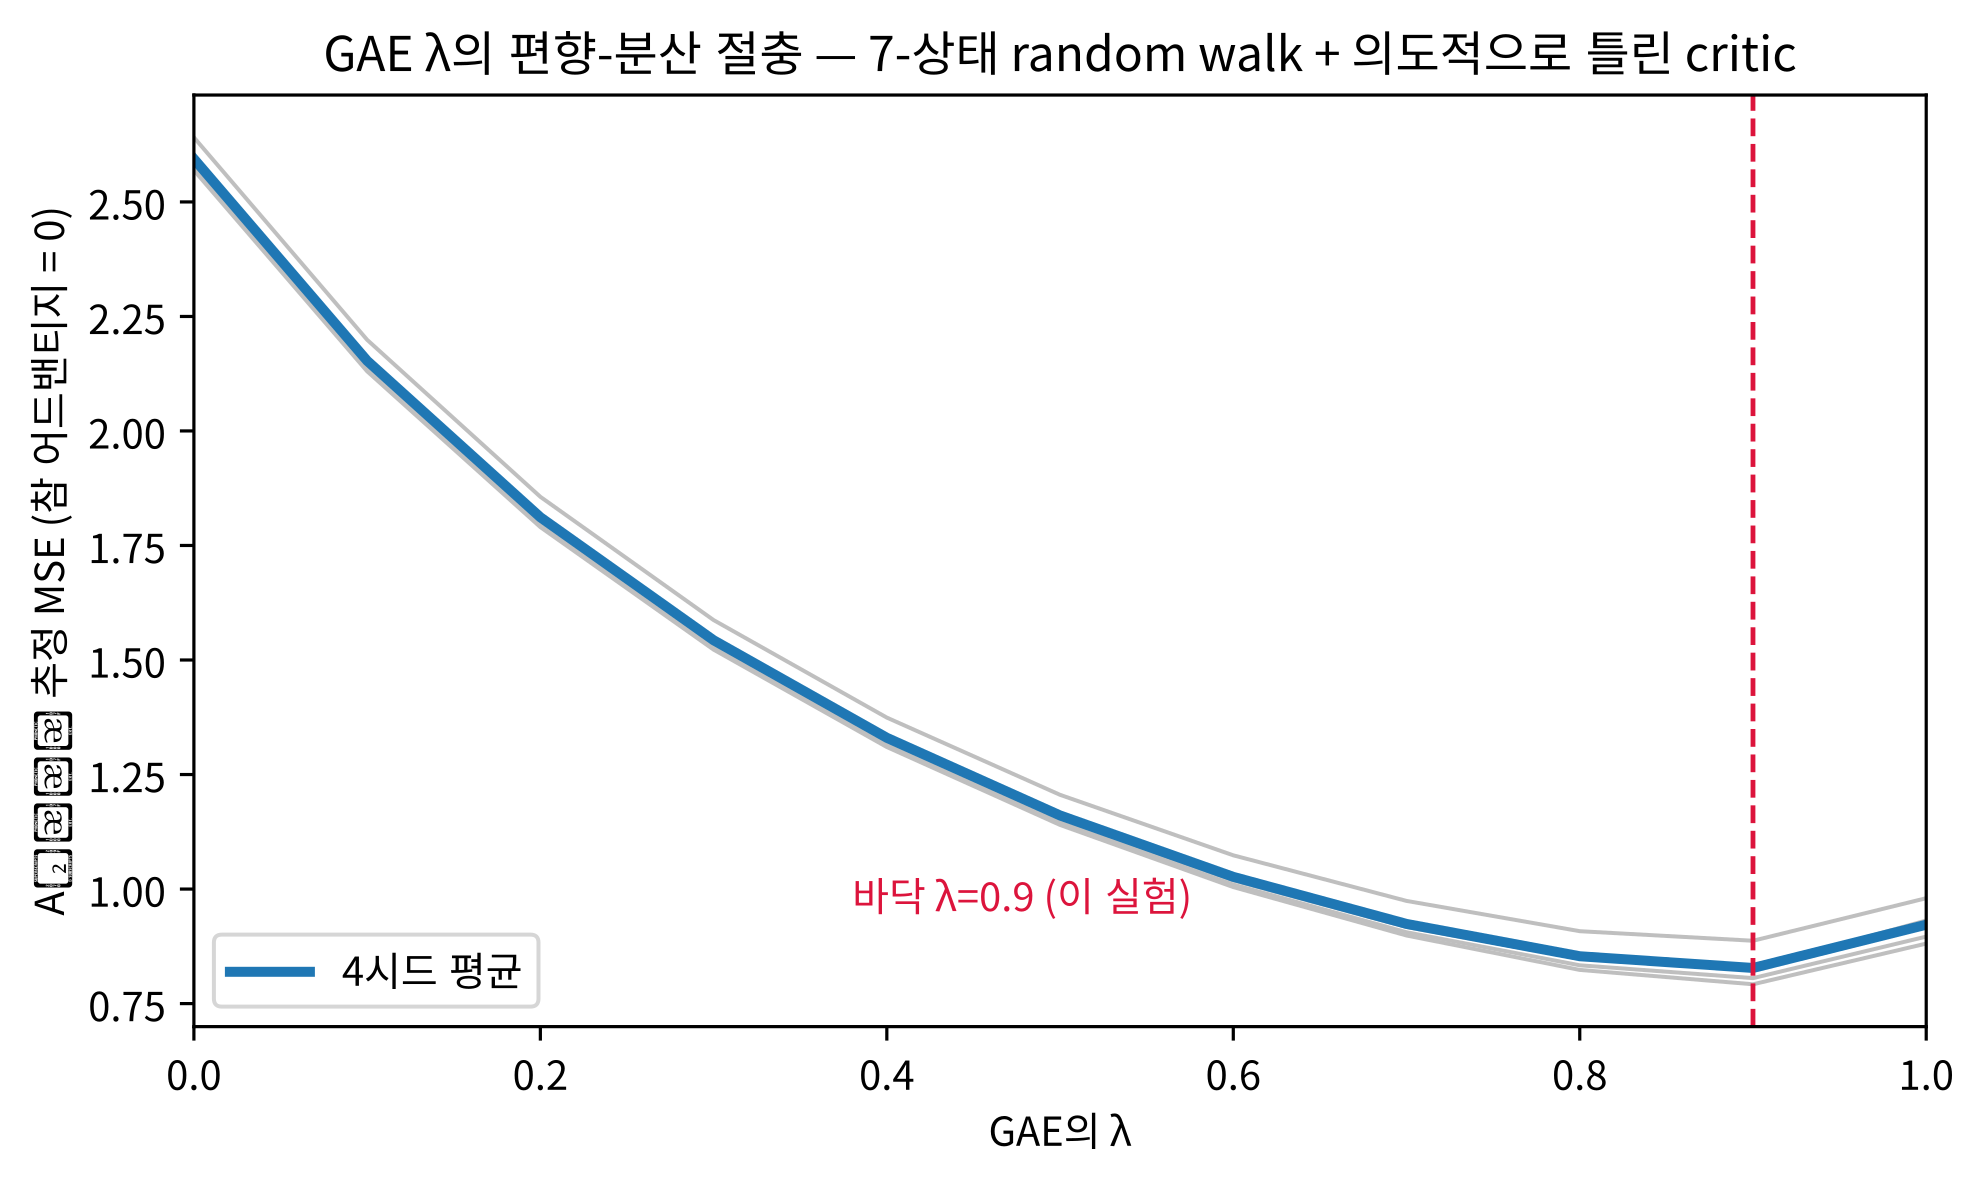
\includegraphics[width=\linewidth]{ch11_3_gae_lambda_ucurve.png}
      {\footnotesize $\lambda=0$(TD 기반, 편향$\uparrow$분산$\downarrow$)
      에서 $\lambda=1$(MC 기반, 편향$\downarrow$분산$\uparrow$)
      사이의 U자 곡선.}
    \end{column}
    \begin{column}{0.40\textwidth}
      {\small
      \kb{실험}(실습 1$\sim$3절): 참값이 정확히 알려진
      7-상태 random walk(7.2절과 같은 환경)에서, \textbf{의도
      적으로 약간 틀린 critic}으로 TD 오차를 만들어
      $A^{\mathrm{GAE}}$ 를 추정 — 참 어드밴티지가 0이므로
      MSE가 곧 ``편향$^2$+분산''.
      \begin{itemize}
        \item $\lambda$ 를 0$\to$1로 훑으면 MSE가 \textbf{U자},
          바닥은 이 환경에서 $\lambda\approx0.9$ 부근.
        \item $n$-step 어드밴티지로 같은 실험이면 바닥
          $n\approx3$ — GAE는 ``n을 고정하고 $\lambda$ 를
          조정''하는 일반화.
      \end{itemize}
      }
    \end{column}
  \end{columns}
  \vskip0.4em
  {\small \kb{7.2절의 교훈이 여기서도 그대로}: 단일 실행(단일
  시드)으로 최적 $\lambda$ 를 정하면 안 된다 — 여러 시드의
  평균으로 U자를 확인한 뒤, 바닥 근처 ``0.90$\sim$0.99''
  사이의 값을 고르면 대체로 안전.}
\end{frame}

\begin{frame}[fragile]{GAE 코드: 뒤에서부터 한 번만 스캔}
  무한합을 그대로 쓰면 각 $t$ 마다 $O(T)$ 합 $\to$ $O(T^2)$.
  재귀를 쓰면 \textbf{뒤에서 앞에서 한 번만} 스캔:
  \begin{lstlisting}
def compute_gae(rewards, values, gamma=0.99, lam=0.95, last_value=0.0):
    T = len(rewards)
    gae, advantages = 0.0, [0.0] * T
    for t in reversed(range(T)):
        next_non_terminal = 1.0 if t < T - 1 else 0.0   # 터미널이면 0
        delta = rewards[t] + gamma * values[t+1] * next_non_terminal \
                - values[t]                              # δ_t
        gae = delta + gamma * lam * next_non_terminal * gae   # 재귀
        advantages[t] = gae
    return advantages
  \end{lstlisting}
  \vskip0.2em
  \small
  \[
  A_t^{\mathrm{GAE}}
  = \delta_t + \gamma\lambda\, A_{t+1}^{\mathrm{GAE}}
  \]
  ``지금의 TD 오차 + 할인된 미래 GAE'' —
  \texttt{gae = delta + gamma * lam * gae} 한 줄이 바로 이
  재귀식. \kb{\texttt{next\_non\_terminal}}: 터미널 상태 도달 시
  ``마지막 값'' 0 처리 (그 뒤에 ``계속될 에피소드''가 없음).
  \texttt{last\_value=0.0} = \textbf{에피소드가 끝난 뒤}의 값;
  에피소드가 끝나지 않고 스텝 버퍼가 가득 찼다면 현재 정책으로
  $V(s_T)$ 계산 (실습 5절 \texttt{collect} 가 이 둘을 구분).
  \begin{block}{GAE로 계산한 $A_t$ 는 미니배치 단위로 정규화}
    $\big((A-\mathrm{mean})/(\mathrm{std}+10^{-8})\big)$ 한 뒤
    클리핑 목적함수에 씀 (11.2절 \texttt{ppo\_clip\_loss}).
    역할은 10.2절 리턴 정규화와 동일 — 정규화하면
    \kb{학습률이 보상 스케일에 무관하게} 작동.
  \end{block}
\end{frame}

\begin{frame}{GAE의 두 가지 ``자주 하는 실수''}
  \small
  \begin{enumerate}
    \item \kb{부호/위치 오류}: \texttt{delta}를
      $r_t+\gamma V(s_t)-V(s_{t+1})$ 으로 쓰면(좌변·우변
      뒤집음) \textbf{모든 어드밴티지의 부호가 반전}되어
      정책이 \textbf{역으로} 학습.
      \smallskip
      {\footnotesize TD 오차 정의 = ``실제로 벌어진 것
      ($r_t+\gamma V(s_{t+1})$)''에서 ``예측한 것
      ($V(s_t)$)''을 뺀 것 — 6.1절과 대조하며 항상 한 번
      확인.}
    \item \kb{last value 0 처리 vs 정책 값 처리 혼동}:
      \texttt{last\_value}는 *에피소드가 끝난 뒤*의 값.
      \begin{itemize}
        \item 에피소드가 끝났다면(터미널) $\to$ \textbf{0}.
        \item 끝나지 않고 스텝 버퍼가 가득 찼다면 $\to$
          \textbf{현재 정책으로} 마지막 상태의 $V(s_T)$ 계산.
      \end{itemize}
      ``끝나지 않았는데 0 대입''하면, 좋은 상태일수록 마지막
      스텝의 $\delta$ 가 음수로 과대평가(가치를 0으로 낮게
      보는 셈)되어 정책이 끝 상태의 좋은 상태를 피하게 됨 —
      학습이 느려지는 원흉 중 하나.
  \end{enumerate}
\end{frame}

\begin{frame}{엔트로피 보너스: 탐험을 유지하는 작은 항}
  \small
  11.2절 실습의 \texttt{GaussianPolicy} 는
  $\mathrm{exp}(\texttt{log\_std})$ 를 \textbf{학습 가능한}
  파라미터로 두었는데, 무엇이 \texttt{log\_std}를 줄여(탐험을
  줄여) 갈까? 답은 세 번째 항:
  \[
  L^{\mathrm{PPO}}(\theta) = \mathbb{E}_t[L^{\mathrm{CLIP}}_t]
  - c_v\,\mathbb{E}_t[(V_\theta(s_t)-R_t)^2]
  + c_e\,\mathbb{E}_t\Big[\underbrace{
  \mathcal{H}\big[\pi_\theta(\cdot\mid s_t)\big]}_{\text{엔트로피
  보너스}}\Big]
  \]
  \begin{itemize}
    \item 세 항: \kb{클리핑 항}(정책 = actor) +
      \kb{Critic TD/리턴 손실}($V$ 를 어드밴티지 계산에 쓸 만큼
      정확히 학습해야 GAE가 의미 있음) + \kb{정책 엔트로피}
      더하기.
    \item 클리핑은 ``한 스텝의 이동''을 막는 \textbf{장치}일 뿐 —
      정책이 \textit{천천히}도 특정 행동에 확률을 1로 몰아붙일
      수 있다. \kb{탐험 소실(exploration collapse)}: 한 번
      확률이 0에 가까워진 행동은 다시 샘플링될 기회가 없어
      \textbf{영원히} 돌아오지 못함.
    \item 엔트로피 $\mathcal{H}[\pi(\cdot\mid s)]
      = -\sum_a \pi(a\mid s)\log\pi(a\mid s)$ 는 ``정책이
      얼마나 불확실한가(균등하면 최대)'' — 최대화하면
      \kb{단일 행동에 수렴하는 것을 구조적으로 늦춤},
      ``한 행동에 확률을 몰아붙이지 마라''는 연료.
  \end{itemize}
  \begin{block}{$c_e$ 는 보통 $0.001\sim0.01$ — 작게}
    크게 하면 ``무작위에 가까운 정책''을 장려해 성능 오히려
    나빠짐. 가우시안 정책에서는 $\sigma$ 가 클수록 엔트로피가
    커지므로 이 항이 바로 \texttt{log\_std}를 \textbf{올려}
    주는 힘. 실전: \texttt{log\_std}를 점진적으로 줄여 가는
    (annealing) 방식도 함께 — ``처음엔 많이 탐험, 수렴하면
    줄여간다''. 11.2절 Pendulum이 아주 느렸던 이유 중 하나는
    바로 이 탐험 신호의 부재(또는 부족).
  \end{block}
\end{frame}

\begin{frame}{TRPO의 한 스텝이 왜 무거운가}
  \small
  PPO 이전에 같은 문제(너무 큰 업데이트로 인한 정책 붕괴)를
  풀던 \kb{TRPO}(2015): KL 제약을 명시적으로 걸고 2차 미분
  도구로 최적화 — 한 스텝은 세 단계.
  \begin{enumerate}
    \item \kb{KL 제약}
      $\mathbb{E}_t[D_{\mathrm{KL}}(\pi_{\theta_{\mathrm{old}}}
      \,\|\,\pi_\theta)]\le\delta$ 를 \textit{명시적으로}
      해석 — 2차 근사(피셔 정보 행렬
      $F=\mathbb{E}[\nabla\log\pi\,\nabla\log\pi^{\top}]$)
     까지 쓰면 이 제약 아래 최대화는 $F$ 의 \textbf{역행렬 곱}을
      구해야 하는 \kb{최대제곱(정준경로) 문제}.
    \item $F$ 는 파라미터 수 $p$ 의 $p\times p$ 행렬 —
      신경망 정책에서 $p$ 가 수만$\sim$수십만, \textbf{직접
      역행렬은 불가}. ``피셔-벡터 곱만 계산할 수 있으면 된다''
      는 성질을 이용해 \kb{conjugate gradient}(반복법)로 근사 해.
    \item 근사해도 \textit{제약이 실제로} 만족되는지 확인 —
      \kb{line search}(제안 방향으로 얼마나 가도 안전한지).
  \end{enumerate}
  세 단계 모두 ``정책 그래디언트'' 자체와 무관한
  \kb{최적화 장치}.
\end{frame}

\begin{frame}{TRPO $\to$ PPO: 기계장치를 클리핑 한 줄로}
  \begin{itemize}
    \item PPO는 이 세 단계를 \kb{클리핑 한 줄}로 대체:
      \[
      \min\Big(r_tA_t,\;
      \mathrm{clip}\big(r_t,1-\epsilon,1+\epsilon\big)A_t\Big)
      \]
      $r_t$ 가 $[1-\epsilon,1+\epsilon]$ 범위를 벗어나면 밖으로
      나간 만큼의 이득을 깎아버리는 \kb{모노토닉 근사}.
    \item TRPO의 ``단조 개선 \textbf{보장}''은 2차 근사 + line
      search가 \textbf{정확히} 동작할 때만 성립 — PPO는 그
      보장을 \textbf{포기}하고 ``보장이 안 되더라도 실전에서 잘
      작동한다''는 경험적 증거로 승부.
  \end{itemize}
  \vskip0.5em
  \begin{block}{구현 비용이 곧 채택의 차이}
    TRPO 참고 구현: 약 \textbf{300$\sim$400줄}(피셔-벡터 곱,
    conjugate gradient, line search 포함). PPO: \textbf{100줄
    안팎}. ``같은 성능에 3배 적은 코드''가 아니라,
    \kb{``대부분의 환경에서 충분히 좋은 성능에 3배 적은
    코드''} — 연구실마다 TRPO 장치를 디버깅하는 시간 대신
    PPO를 그냥 돌려보는 쪽으로 기울 수밖에 없었다.
  \end{block}
\end{frame}

\begin{frame}{역사적 일화: PPO-Clip vs PPO-Penalty}
  \begin{itemize}
    \item PPO 논문(2017)은 실제로 TRPO를 ``더 단순하게'' 하고
      싶다는 시도에서 출발 — 같은 연구팀(OpenAI, Schulman 외)이
      먼저 TRPO(2015)로 ``신뢰 영역'' 개념을 세웠고, 다음
      질문: ``KL 제약을 풀어내는 그 무거운 최적화 없이,
      \textbf{클링(=클리핑)만으로} 비슷한 안정성을 얻을 수
      있는가?''
    \item 논문에서는 클리핑(PPO-Clip) 외에도 \kb{KL
      페널티} 방식(PPO-Penalty: KL이 크면 목적함수에 벌을
      부과)을 함께 제안.
    \item PPO-Penalty는 KL 벌의 계수를 \textbf{학습 중 동적으로
      조정}해야 함 (너무 크면 탐험 부족, 너무 작으면 클리핑
      없이 폭주) — \kb{PPO-Clip 쪽이 훨씬 실용적}이라 실전에서
      사실상 표준이 됨.
  \end{itemize}
  \vskip0.5em
  \begin{block}{``PPO = 클리핑''이라는 현재 통념의 기원}
    이 선택의 결과 — ``보장을 근사로'' 바꾼 것이 이긴 드문
    경우.
  \end{block}
\end{frame}

\begin{frame}{PPO는 TRPO보다 ``나쁜'' 알고리즘인가?}
  \kq{아니다 — ``이론적 보장이 약하고, 실전 성능은
  비견되는'' 알고리즘.}
  \vskip0.6em
  \begin{itemize}
    \item TRPO의 단조 개선은 2차 근사 + line search의
      \textbf{정확성}에 의존 — 실전(큰 네트워크, 미니배치
      샘플 노이즈)에서는 그 근사 자체가 충분히 정확하지 않음.
    \item 즉 \kb{TRPO의 ``보장''도 실전에서는 이론만큼 강하지
      않다} — PPO가 ``보장을 포기''하는 대가는 생각보다
      작았고, \textbf{구현 단순성}이라는 이득은 컸다. 이것이
      ``표준이 된 이유''의 첫 번째 축.
  \end{itemize}
  \vskip0.5em
  \begin{block}{이 실용성 덕분에}
    PPO는 지금 \kb{가장 널리 쓰이는 정책기반 알고리즘} — 로봇
    보행 제어, OpenAI Five(Dota 2, 2019), AlphaStar(스타크래프트
    II, 2019)뿐 아니라, \textbf{RLHF}(인간 피드백으로
    언어모델 조정)의 핵심 도구로도.
    \kb{연속 제어(로봇의 관절 힘)와 이산 선택(다음 토큰 고르기)
    양쪽 모두에 그대로 적용}될 만큼 범용적.
  \end{block}
\end{frame}

\begin{frame}{``범용적''이라는 말의 구체적 의미}
  PPO의 목적함수는 \kb{행동공간이 이산이든 연속이든 같은
  형태}.
  \vskip0.5em
  \begin{columns}[T]
    \begin{column}{0.5\textwidth}
      \kb{이산} (CartPole, 언어모델의 토큰 선택)
      \begin{itemize}
        \item $\pi$ 가 $\mathrm{softmax}$.
        \item $\log\pi(a\mid s)$ 는 Categorical 분포의
          로그확률.
        \item 행동은 \texttt{argmax} 대신 \textbf{샘플링}
          (10.2절
          \texttt{torch.distributions.Categorical}).
      \end{itemize}
    \end{column}
    \begin{column}{0.5\textwidth}
      \kb{연속} (Pendulum, 로봇 관절)
      \begin{itemize}
        \item $\pi$ 가 \textbf{가우시안}
          $\mathcal{N}(\mu_\theta(s),\,\sigma_\theta^2 I)$.
        \item $\log\pi(a\mid s)$ 는 정규분포의 로그우도.
        \item 행동은 \texttt{dist.sample()} (11.2절
          \texttt{GaussianPolicy}).
      \end{itemize}
    \end{column}
  \end{columns}
  \vskip0.7em
  \begin{block}{점}
    목적함수 $\mathbb{E}[L^{\mathrm{CLIP}}]$ 과 GAE, 엔트로피 항의
    \textbf{수학적 형식은 같다} — 변하는 건 ``$\log\pi$ 를 어떤
    분포에서 계산하느냐''뿐. (11.2절 FAQ의 ``연속 정책이
    $\mathrm{tanh}$ 로 스케일되는 이유''도 이 맥락: 가우시안의
    지지공간이 실수 전체인데 실제 환경은 행동 범위가
    $[-1,1]$ 같이 제한 → $\mathrm{tanh}$ 로 압축.)
  \end{block}
\end{frame}

\begin{frame}{``PPO를 돌린다'' — 실전 스택의 전체 그림}
  \small
  PPO 한 반복(1 iteration)이 실제로 하는 일, 위에서 아래로:
  \vskip0.3em
  \begin{enumerate}
    \item \kb{① 경험 수집}: 현재 정책 $\pi_{\theta_{\mathrm{old}}}$
      으로 $N$ 스텝(예: 2048) 수집 — 스텝마다 $s_t,\ a_t,\ r_t,\
      \log\pi_{\theta_{\mathrm{old}}}(a_t\mid s_t),\
      V_{\theta_{\mathrm{old}}}(s_t)$ 저장.
    \item \kb{② last value 계산}: 마지막 상태의 $V$ 값.
    \item \kb{③ compute\_gae}: 각 스텝의 $A_t$
      ($\lambda=0.95,\ \gamma=0.99$).
    \item \kb{④ 정규화}: $A_t$ 를 미니배치 단위로
      (mean 0, std 1).
    \item \kb{⑤ $M$ epochs}(예: 4) 동안 미니배치(예: 64)마다 경사
      상승: 정책 손실 $=-\min(r_tA_t,\ \mathrm{clip}(r_t,1\pm
      \epsilon)A_t)$ ($\epsilon=0.2$) + Critic 손실
      $\mathrm{MSE}(V_\theta(s_t),R_t)$ ($R_t=A_t+V(s_t)$)
      $-c_e\,\mathcal{H}[\pi_\theta]$.
    \item \kb{⑥ $\theta_{\mathrm{old}}\leftarrow\theta$}:
      다음 반복의 기준 정책 갱신 $\to$ ①로.
  \end{enumerate}
\end{frame}

\begin{frame}{스택의 각 단계 ``왜 이렇게''}
  \small
  \begin{itemize}
    \item \kb{① $N$ 스텝}: 너무 크면 수집 \textit{중에도} 초기·
      말기 정책이 달라져 $r_t$ 가 클리핑 범위를 벗어나는 스텝
      증가; 너무 작으면 GAE의 ``긴 지평선'' 이득 감소.
      실전 $N=2048,\,4096$ 일반적.
    \item \kb{③ GAE($\lambda=0.95$)}: 10.3절의
      $A_t=G_t-V(s_t)$ ($=\lambda1$, MC)를 \textbf{대신} —
      ``거의 MC인데, 가장 먼 꼬리는 약간 얕게 본다''.
    \item \kb{④ 정규화}: 학습률을 보상 스케일에 무관하게 —
      \textbf{미니배치 단위}여야 함. 전체 $N$ 스텝 단위로 하면
      미니배치마다 스케일이 달라져(일부 미니배치의 $A$ 가 0에
      가까워져) 그 업데이트가 거의 사라짐.
    \item \kb{⑤ $M$ epochs}: on-policy(REINFORCE)는 데이터 1회.
      PPO는 클리핑 덕분에 ``데이터가 약간 오래돼도'' 안전하게
      재사용 — $M$ 번(보통 4$\sim$10). $M$ 이 크면 on-policy에
      가깝고(데이터 활용도$\uparrow$) 클리핑 더 자주 발동.
      \textbf{$M=1$ 이면 사실상 A2C/A3C(10.3절)}와 같음.
    \item \kb{⑥ $\theta_{\mathrm{old}}$ 갱신}: 다음 반복에서
      $r_t$ 의 분모가 \textit{이번 반복 끝}의 정책이 되도록 —
      비율이 의미 있게 (1 근처에) 유지.
  \end{itemize}
  {\footnotesize 이 스택의 \textbf{모든 숫자}($N,\ M,\ \epsilon,\
  \lambda,\ \gamma,\ c_v,\ c_e$, 학습률)가 하이퍼파라미터 —
  ``PPO가 느리다/잘 못 배운다''는 불만의 상당 부분이
  \textit{알고리즘이 아니라 이 숫자 조합}에서 옴.
  $\epsilon$ 과 $\lambda$ 는 독립적이지만 \textbf{함께}
  학습 안정성에 영향.}
\end{frame}

\begin{frame}{PPO 한 반복의 전체 데이터 흐름}
  \begin{columns}[T]
    \begin{column}{0.60\textwidth}
      \centering
      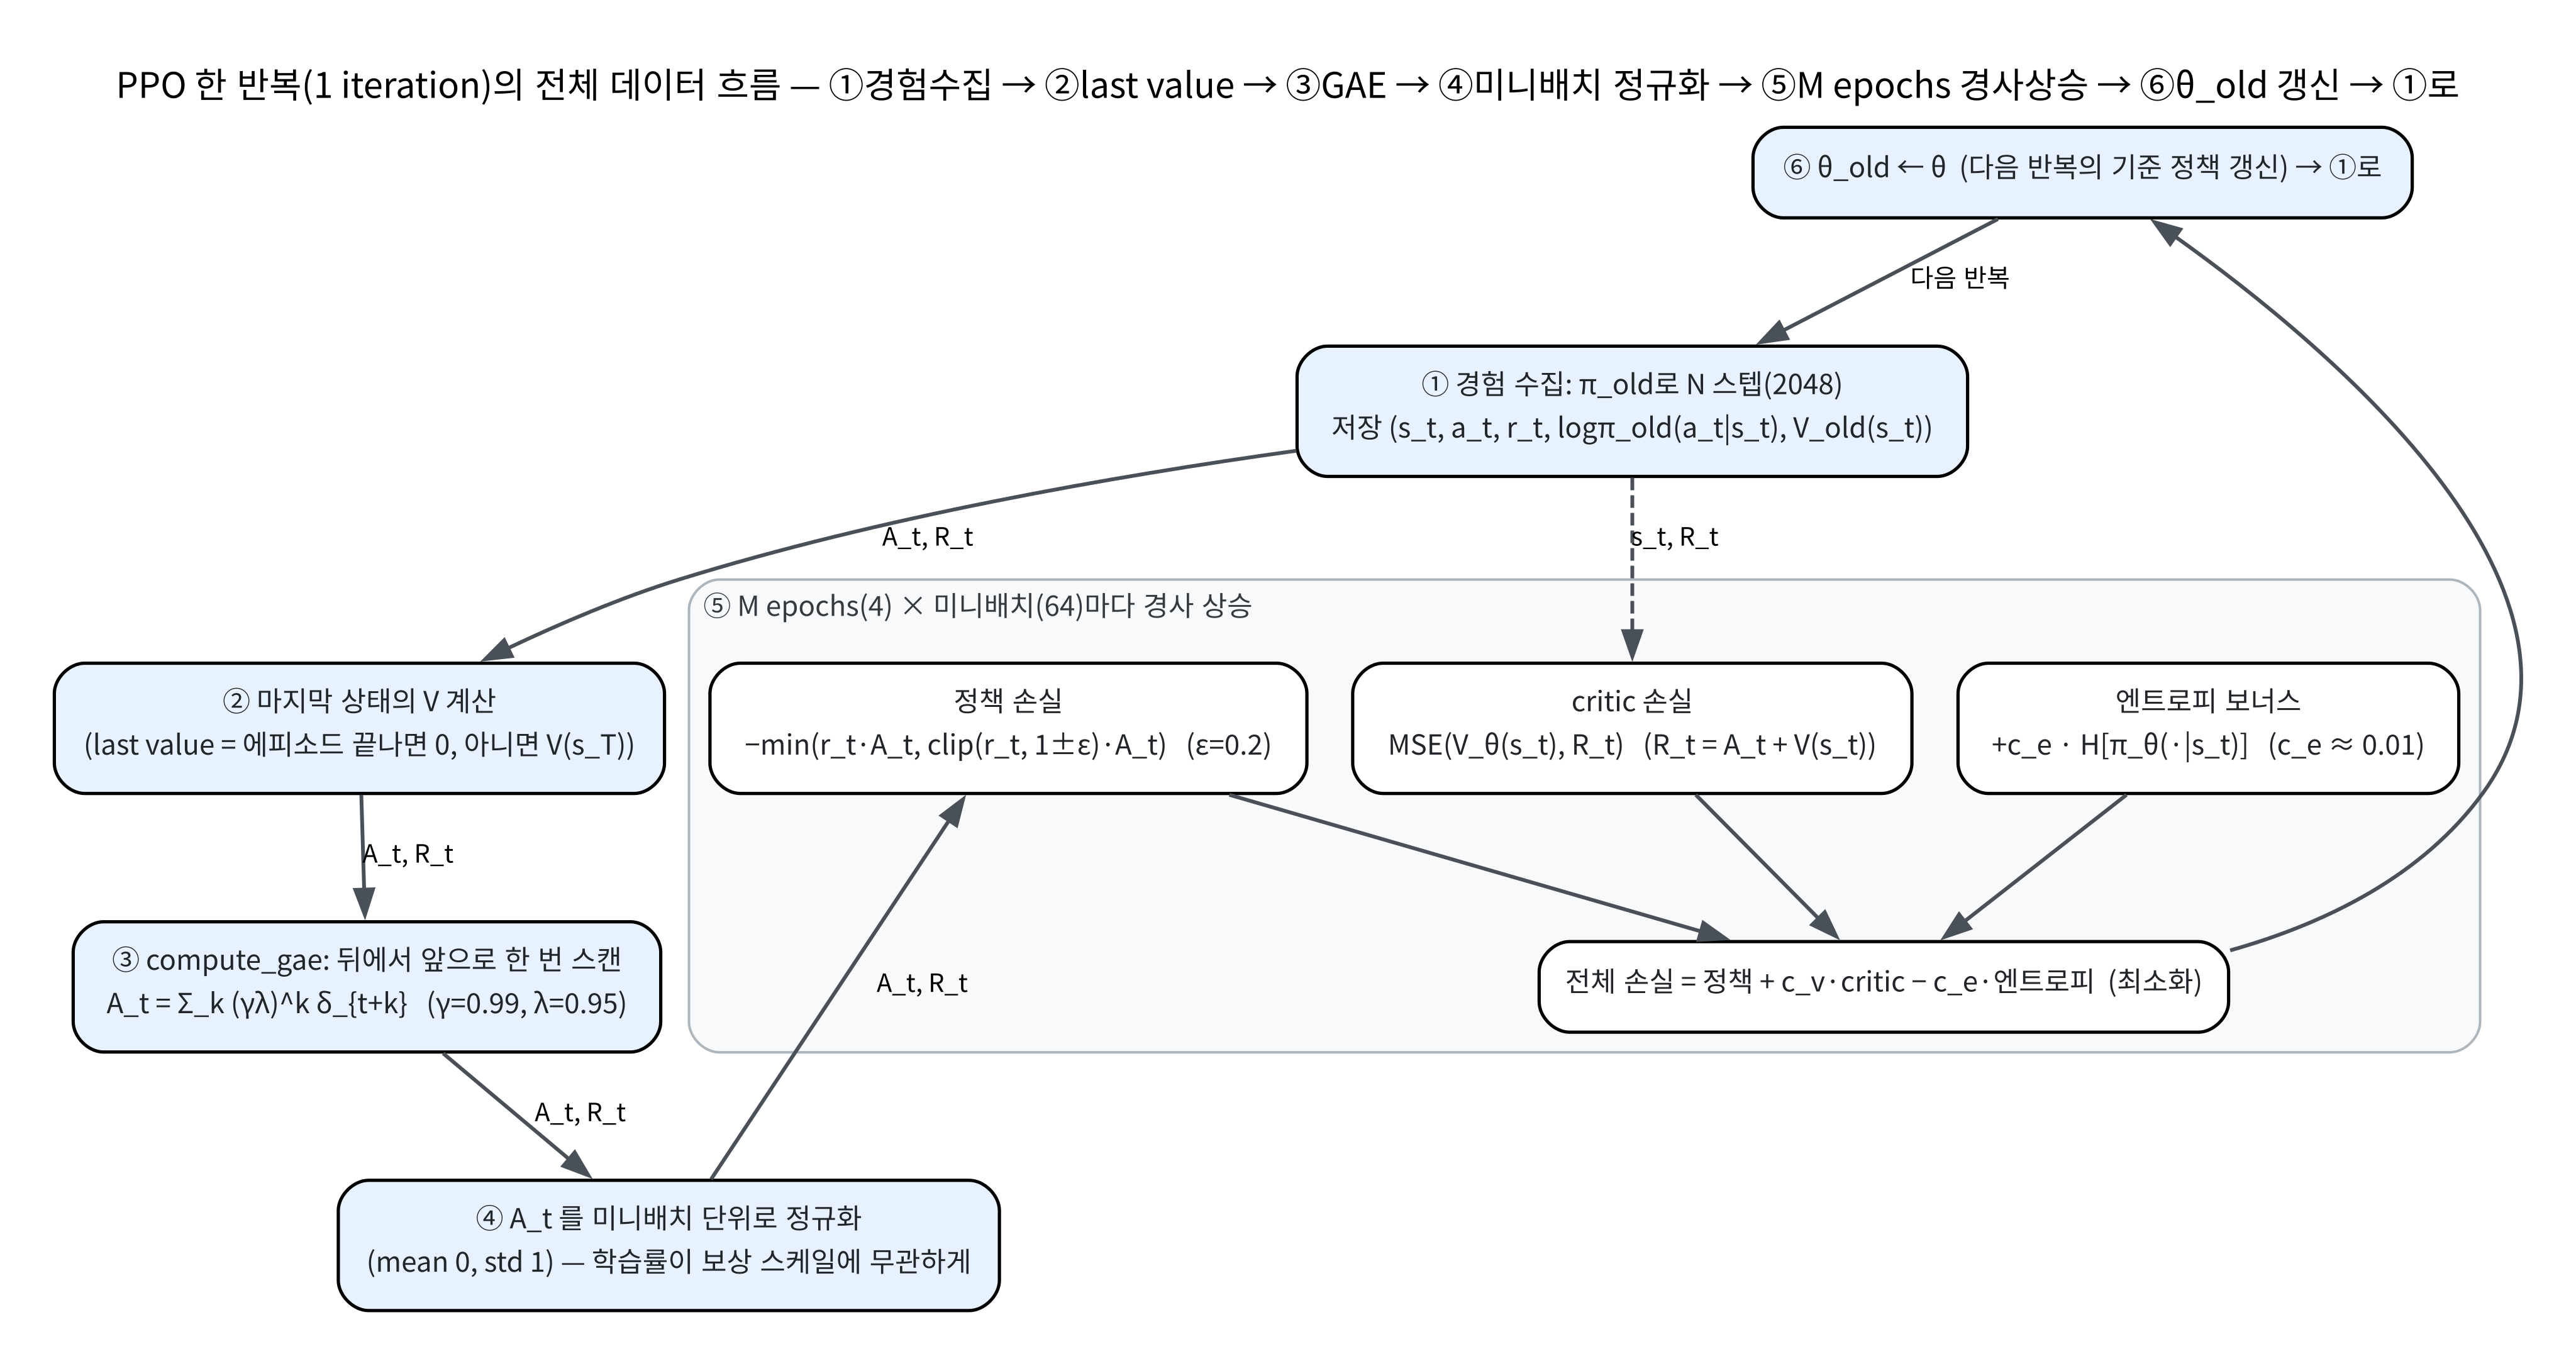
\includegraphics[width=\linewidth]{ch11_3_ppo_pipeline.png}
      {\footnotesize experience buffer가 GAE와 Critic 손실,
      정책 손실(클리핑)로 분기, 엔트로피 항이 정책 손실에 더해지는
      구조.}
    \end{column}
    \begin{column}{0.38\textwidth}
      {\small
      ①경험수집 $\to$ ②last value $\to$ ③GAE $\to$ ④정규화
      $\to$ ⑤$M$ epochs 미니배치 경사상승 $\to$ ⑥
      $\theta_{\mathrm{old}}$ 갱신.
      \\[0.8em]
      11.2절의 골격 + 11.3절의 GAE·엔트로피 = \textbf{실전
      스택}.
      }
    \end{column}
  \end{columns}
\end{frame}

\begin{frame}{실습: CartPole에서 $\lambda$ 를 바꿔가며 PPO}
  이론 검증 — CartPole(이산 행동)에서 PPO를 \kb{$\lambda$ 를
  바꿔가며} 학습, GAE의 절충점을 눈으로 확인. 11.2절
  Pendulum(연속, 30만 스텝에도 $-1092$)과 달리 CartPole은
  이산 보상(매 스텝 $+1$, 최대 500)이라 \textbf{5만 스텝
  안에도} 명확한 차이.
  \vskip0.5em
  세 가지 $\lambda$ — 0.0 (TD(0) 기반, 편향$\uparrow$분산$\downarrow$),
  0.95 (실전 기본값), 1.0 (MC 기반, 편향$\downarrow$분산$\uparrow$) —
  을 \textbf{같은 시드(0), 같은 반복 수}(150$\times$512 스텝
  $\approx$ 7.7만 스텝)로.
  \vskip0.6em
  \small
  \begin{tabular}{@{}lrrrl@{}}
    \toprule
    $\lambda$ & 처음20 리턴 & 마지막20 리턴 & 최고 리턴 &
      20에피소드 평가 (평균/최고) \\
    \midrule
    0.0 (TD) & 55.7 & 126.5 & 270 & 272 / 301 \\
    0.95 (기본) & 29.8 & 141.2 & 442 & 274 / 317 \\
    1.0 (MC) & 26.1 & 169.1 & 449 & \textbf{500 / 500} \\
    \bottomrule
  \end{tabular}
\end{frame}

\begin{frame}{$\lambda$ 학습 곡선 비교 — ``모양''이 달라짐}
  \begin{columns}[T]
    \begin{column}{0.56\textwidth}
      \centering
      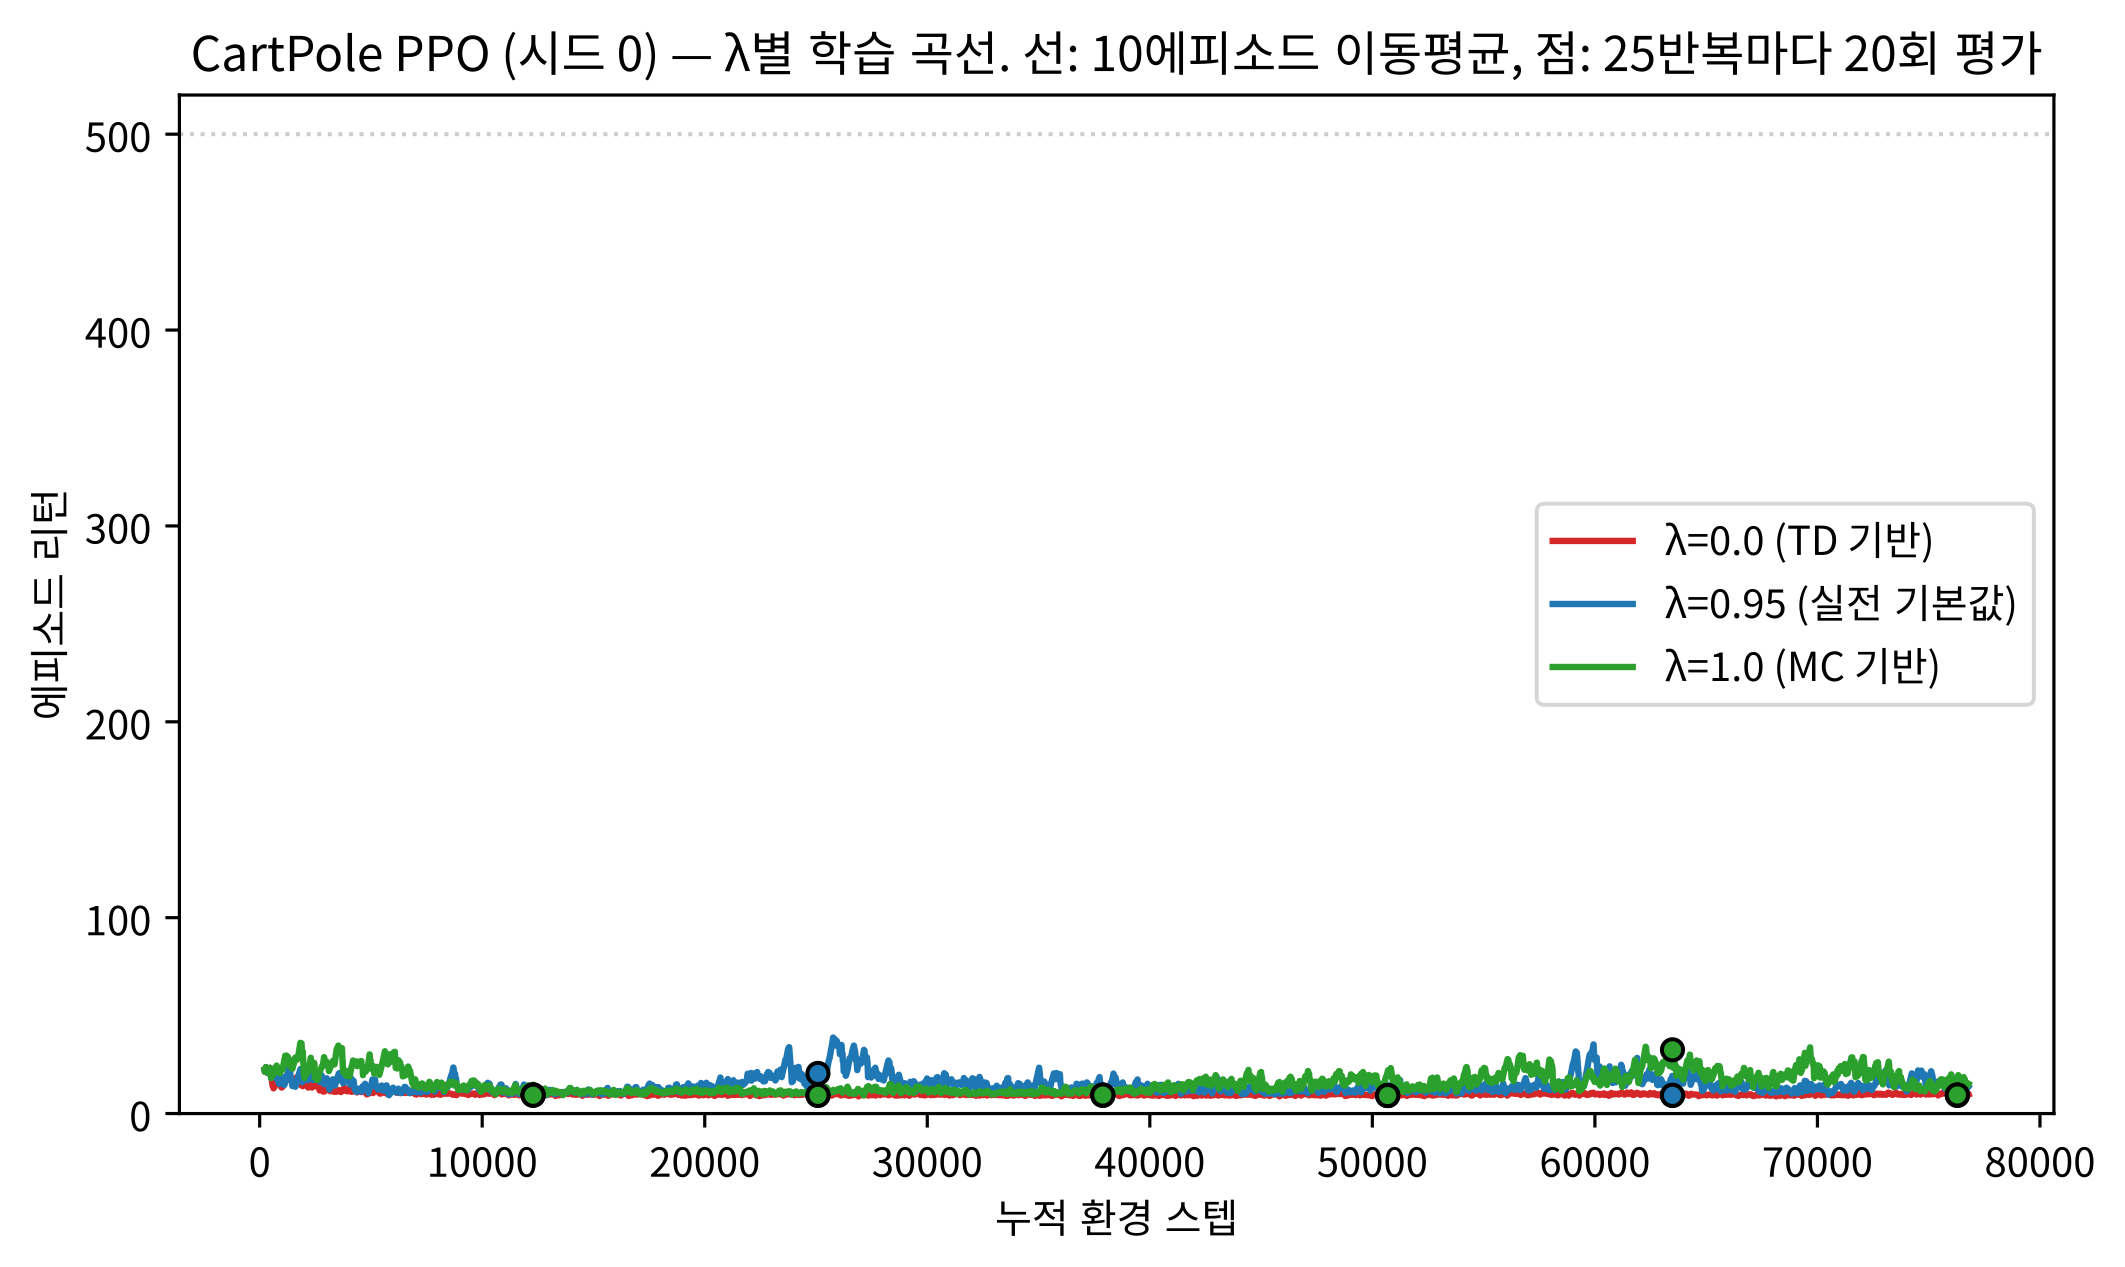
\includegraphics[width=\linewidth]{ch11_3_ppo_lambda_cartpole.png}
      {\footnotesize CartPole, $\lambda=0.0/0.95/1.0$ PPO 학습
      곡선 비교 (시드 0, 150$\times$512 스텝).}
    \end{column}
    \begin{column}{0.42\textwidth}
      {\small
      이번 단일 실행에서 세 $\lambda$ 가 각각 다른
      \textit{모양}으로 학습:
      \begin{itemize}
        \item $\lambda=0.0$: 가장 \textbf{빠르게 시작}
          (처음20 = 55.7)하지만 100 반복 이후 100$\sim$140 대
         에서 \textbf{정체}(최고 270) — ``지금의 TD 오차''만
          믿는 편향이 방향을 자주 틀리게 하는 흔적.
        \item $\lambda=1.0$: 시작은 느렸지만 \textbf{후반에
          가장 멀리}(마지막20 = 169.1), 평가 20개 에피소드
          \textbf{모두 500}(만점).
        \item $\lambda=0.95$: 어느 지표에서도 단연 우월하지
          않지만, \textbf{어디 하나 치명적 결함도 없음}.
      \end{itemize}
      }
    \end{column}
  \end{columns}
  \vskip0.4em
  {\small \kb{중요}: 단일 시드 실험이므로 ``$\lambda=0.95$ 가
  항상 이긴다''(또는 ``1.0이 이긴다'')는 \textbf{보장은
  없다} — 7.2절의 교훈처럼 여러 시드로 평균해야 한다. 이번
  실습은 ``$\lambda$ 에 따라 학습의 \textit{모양}이 달라지는
  절충의 존재''를 보는 것이지, 어느 $\lambda$ 가 \textit{최적}
  인지를 증명하는 것이 아니다.}
\end{frame}

\begin{frame}{자주 묻는 질문 — GAE와 PPO의 하이퍼파라미터}
  \small
  \begin{itemize}
    \item \kb{Q. GAE의 $\lambda$ 와 클리핑의 $\epsilon$ 은
      독립적?} 역할은 다르지만 \textbf{함께} 학습 안정성에 영향 —
      $\lambda$ 는 ``어드밴티지 추정 \textit{자체}의
      편향-분산'', $\epsilon$ 은 ``그 추정을 바탕으로 정책을
      얼마나 크게 바꿀 것인가''. 어드밴티지 추정이 노이즈가
      크면($\lambda$ 가 1에 가까우면) 클리핑이 그 노이즈로부터
      정책을 \textbf{보호}하는 역할이 더 중요 — 실전에서는 둘
      함께 튜닝.
    \item \kb{Q. RLHF에서 PPO는 무엇을 ``행동''으로 보나?}
      언어모델을 정책으로 볼 때 \kb{상태} = 지금까지 생성된
      토큰들, \kb{행동} = 다음에 고를 토큰, \kb{보상} =
      보상모델의 점수. 토큰 하나하나를 고르는 것이 이산 행동
      선택이므로 이번 장의 \textbf{이산 행동공간 PPO가 사실상
      그대로 적용} — 로봇(연속)과 언어모델(이산)이라는 완전히
      다른 응용에 같은 알고리즘이 쓰이는 것 자체가 ``행동공간
      형태에 크게 의존하지 않는'' 범용성의 증거.
    \item \kb{Q. GAE의 $\lambda$ 와 7절 적격흔적 TD($\lambda$)의
      $\lambda$ 는 같은 것인가?} ``같은 아이디어''지만
      \textbf{적용 대상이 다름} — 적격흔적의 $\lambda$ 는
      \textit{가치함수 $V$}의 갱신에 ``어떤 $n$-step TD를
      가중합할지'', GAE의 $\lambda$ 는 \textit{어드밴티지
      $A_t$}를 ``어떤 $n$-step 어드밴티지를 가중합할지'' 결정.
      수학적 구조(지수 가중 $\lambda^k$ 의 합)는 같음 —
      적격흔적은 critic 학습에, GAE는 actor의 어드밴티지
      계산에.
    \item \kb{Q. 엔트로피 $c_e$ 를 너무 크게?} ``무작위에
      가까운 정책''이 장려되어, 좋은 행동을 찾았을 때도 확률을
      높이지 못해(엔트로피 최대화가 ``균등한 확률''을 유지하려
      함) 성능 오히려 나빠짐 — 실전 $c_e=0.001\sim0.01$ 로
      작게, 끝단계에서 0으로 줄여(annealing) ``탐험 종료''.
  \end{itemize}
\end{frame}

\begin{frame}{이번 주차 정리}
  \begin{itemize}
    \item \kb{11.1 신뢰 영역과 확률비} —
      \begin{itemize}
        \item 신뢰 영역 = 한 걸음의 크기를 ``믿을 수 있는
          범위''(KL 발산)로 제한하는 직관.
        \item 확률비 $r_t=\pi_\theta/\pi_{\mathrm{old}}$ : 첫
          스텝에서는 정직한 policy gradient, $r_t$ 가 크면
          분산 $e^{\mu^2}-1$ 으로 지수적 불어나기 → 소수 극단
          샘플 지배.
      \end{itemize}
    \item \kb{11.2 PPO 클리핑과 연속 제어} —
      \begin{itemize}
        \item 클리핑 한 줄: min의 모서리가 \textbf{개선
          방향에만} 상한(비대칭). 전체 목적함수 = 정책 +
          Critic $-$ 엔트로피.
        \item Pendulum 실습: 연속 제어는 탐색 체적 때문에
          본질적으로 느림(12만 스텝 ≈ 8\% 개선).
      \end{itemize}
    \item \kb{11.3 GAE와 실전 스택} —
      \begin{itemize}
        \item GAE = 여러 시점 TD 오차의 지수 가중합
          ($\lambda$ 로 TD$\leftrightarrow$MC 절충, 기본값
          0.95) + 엔트로피 보너스가 탐험 소실을 늦춤.
        \item TRPO의 300$\sim$400줄 장치를 클리핑 100줄로
          대체 → ``보장은 근사로, 실용성은 그대로'' —
          표준이 된 이유.
      \end{itemize}
  \end{itemize}
  \vskip0.6em
  \begin{block}{PPO 공식}
    \kb{PPO = (11.1 확률비) $\times$ (11.2 클리핑) + (11.3 GAE·
    엔트로피·실전 스택)} — 각각 빠지면 ``폭주(REINFORCE)'',
    ``불안정(클립 없는 IS)'', ``느리고 탐험 소실(GAE/엔트로피
    없음)''.
  \end{block}
  \vskip0.3em
  \begin{block}{다음 주차 — Chapter 12. 모방학습과 인간 피드백}
    보상의 시행착오 대신 \textbf{사람의 시연과 선호}로부터 배우는
    방향 — Chapter 2$\sim$11의 보상 최적화 알고리즘 중 가장
    강한 PPO가 ``왜 보상 최적화만으론 안 되는가''를 비교하기
    위한 기준점이 됨.
  \end{block}
\end{frame}

\end{document}
